
\chapter{Feynman Rules}
\label{chap:fr} %noinstiki
%instiki:
%instiki:***
%instiki:
%instiki:[[Beyond|Contents]]
%instiki:
%instiki:***
%instiki:
%instiki:* [Interaction picture](#interaction-picture)
%instiki:
%instiki:* [Yukawa interaction](#feynman-diagrams)
%instiki:
%instiki:* [Scattering](#scattering)
%instiki:
In progress: The previous chapter will be rewritten in terms of Weyl spinors.

When the case of interacting fields are considered, the particles can be created, destroyed and scattered. In essence this requires solving the coupled non-linear field equations for given conditions. This is an extremely difficult problem which has only been solved in perturbation theory.

In the Heisenberg picture, which we have so far been using, this program is still very complex, and it was decisive for the successful development of the theory to work instead in the interaction picture. In section \ref{sec:interaction-picture} we write the $S$--matrix expansion derived in Chapter~\ref{cha:s-matrix}, in the interaction picture. In section \ref{sec:feynman-diagrams} we show how to use the Wick expansion to calculate $S$--matrix elements involving scalars and spinors.

The considerations which allow to write a formal series of the
evolution operator are completely general and apply just as well the
perturbative calculation of the scattering operator as to the Green
functions of the many-body problem in Appendix~\ref{cha:green-functions}.


\section{Interaction picture}
\label{sec:interaction-picture}
This part is based in \cite{Mandl:1985bg}. 

The system is decribed by a Hamiltonian $H=H_0+H_I$, where $H_{0}$ is the non-perturbated Hamiltonian and $H_I$ is the interaction Hamiltonian (which can depend on time). 

In the Schr\"odinger Picture (SP) the time dependence is carried by the states according to the Scr\"odinger equation 
\begin{align}\
\label{eq:84f}
  i\frac{\partial}{\partial t}|a,t\rangle_{\text{S}}=  i\frac{d}{dt}|a,t\rangle_{\text{S}}=  {H}|a,t\rangle_{\text{S}}
\end{align}
With the solution given in Eq.~\eqref{eq:39f}
\begin{align}
\label{eq:85f}
    |a,t\rangle_{\text{S}}=U(t,t_i)|a\rangle_{\text{S}}\,.
\end{align}
where $U$ is the unitary operator [see Eq.~\eqref{eq:40f}]
\begin{align}
 U\equiv U(t,t_i)= e^{-i H(t-t_i)}\,.
\end{align}
Given the state $|a,t\rangle_{\text{S}}$ in the SP, in the Heisenberg picture (HP) we defined the state
\begin{align}
\label{eq:86f}
  |a\rangle_H=U^\dagger|a,t\rangle_{\text{S}}=|a\rangle_{\text{S}}
\end{align}
Si $O^{\text{S}}$ in an operator in the SP, the corresponding Heisenberg operator is defined as
\begin{align}
\label{eq:87f}
  O^{\text{H}}(t)=U^\dagger O^{\text{S}}U
\end{align}
Hence, the transformation from HP to SP is unitary. At $t=t_i$, states and operators in the two pictures are the same. We see from Eq.~\eqref{eq:86f} that in the HP state vectors are constant in time, while from Eq.~\eqref{eq:87f} the Heisenberg operators evolve with time. Is convenient to keep the temporal label in the Heisenberg states
\begin{align}
  |a\rangle_H=|a,t_i\rangle_H
\end{align}
Eq.~\eqref{eq:87f} ensures the invariance of matrix elements and commutation relations:
\begin{align}
  {}_{\text{S}}\langle b,t|\,O^{\text{S}}\,|a,t\rangle_{\text{S}}=  {}_{\text{S}}\langle b,t|\,U O^{\text{H}}(t) U^\dagger\,|a,t\rangle_{\text{S}}=
{}_{\text{H}}\langle b,t_i|O^{\text{H}}(t)|a,t_i\rangle_{\text{H}}
\end{align}
\begin{align}
\left[O^{\text{S}},P^{\text{S}}\right]=c\Rightarrow\left[O^{\text{H}}(t),P^{\text{H}}(t)\right]=c
\end{align}
where $c$ is a constant.

Differentiation of Eq. \eqref{eq:87f} 
\begin{align}
  \frac{d}{dt}O^{\text{H}}(t)=&\left(\frac{d}{dt}U^\dagger\right)O^{\text{S}}U+
U^\dagger O^{\text{S}}\frac{d}{dt}U\nonumber\\
 =&i H\, U^\dagger O^{\text{S}}U+
U^\dagger O^{\text{S}}U(-i H)\nonumber\\
 =&-i ( O^{\text{H}}H-H O^{\text{H}})\,,
\end{align}
gives the Heisenberg equation of motion

\begin{align}
  i\frac{d}{dt}O^{\text{H}}(t)=\left[O^{\text{H}}(t),H\right]
\end{align}
The interaction picture (IP) arises if the Hamiltonian is split into two parts
\begin{align}
  H=H_0+H_{\text{I}}\,.
\end{align}
In quantum field theory $H_I$ will describe the interaction between two fields, themselves described by $H_0$

IP is related to the SP by the unitary transformation
\begin{align}
\label{eq:88f}
  U_i\equiv U_i(t,t_i)=e^{-i H_i(t-t_i)}\,,
\end{align}
in this way,
\begin{align}
\label{eq:89f}
  |a,t\rangle_{\text{I}}=U_0^\dagger|a,t\rangle_{\text{S}}\,,
\end{align}
and
\begin{align}
\label{eq:90f}
  O^{\text{I}}(t)=U^\dagger_0 O^{\text{S}}U_0\,.
\end{align}
Thus the relation between IP and SP is similar to that between HP and SP, but with the unitary transformation $U_0$ involving only the non--interacting Hamiltonian $H_0$. Note that both the vector states as the operators in the IP are time-dependent.

Differentiating Eq.~\eqref{eq:90f} gives the differential equation of motion operators in the IP:
\begin{align}
  i\frac{d}{dt}O^{\text{I}}(t)=\left[O^{\text{I}}(t),H_0\right]
\end{align}

Substituting Eq.~\eqref{eq:89f} into the Scr\"odinger Eq.~\eqref{eq:84f}, one obtains the equation of motion of state vectors in the IP, If the system is described by a time-dependent state vector $|\Phi(t)\rangle$
\begin{align}
  i\frac{d}{dt}|a,t\rangle_{\text{S}}=&  H^{\text{S}}|a,t\rangle_{\text{S}}\nonumber\\
  i\frac{d}{dt}\left(U_0|\Phi(t)\rangle\right)=&  H^{\text{S}}U_0|\Phi(t)\rangle\nonumber\\
  i\left(\frac{d}{dt}U_0\right)|\Phi(t)\rangle+iU_0\frac{d}{dt}|\Phi(t)\rangle=&  H^{\text{S}}U_0|\Phi(t)\rangle\nonumber\\
  U_0 H_0|\Phi(t)\rangle+iU_0\frac{d}{dt}|\Phi(t)\rangle=&  H^{\text{S}}U_0|\Phi(t)\rangle\nonumber\\
  U_0 H_0|\Phi(t)\rangle+iU_0\frac{d}{dt}|\Phi(t)\rangle=&  (H_0+H_I^{\text{S}})U_0|\Phi(t)\rangle\nonumber\\
  iU_0\frac{d}{dt}|\Phi(t)\rangle=&  H_I^{\text{S}}U_0|\Phi(t)\rangle\nonumber\\
  i\frac{d}{dt}|\Phi(t)\rangle=& U_0 H_I^{\text{S}}U_0|\Phi(t)\rangle
\end{align}
\begin{align}
\label{eq:91f}
  i\frac{d}{d t}|\Phi(t)\rangle_{\text{I}}=H^{\text{I}}_I\,|\Phi(t)\rangle_{\text{I}}\,,
\end{align}
where, as in Eq.~\eqref{eq:90f}
\begin{align}
  \label{eq:92f}
  H^{\text{I}}_I=e^{i H_0^{{\text{S}}}(t-t_i)}H^{\text{S}}_I e^{-i H_0^{{\text{S}}}(t-t_i)}
\end{align}
is the interaction Hamiltonian in the IP, with $H^{\text{S}}_I$ and $H^{\text{S}}_0$ being the interaction and free-field Hamiltonian in the SP. From now on we shall omit the labels I, used in the equations to distinguish the IP, as we shall be working exclusively in the IP in what follows.

Eq. \eqref{eq:91f} is a Scr\"odinger-like equation with the time dependent Hamiltonian $H_I(t)$. With the interaction switched off (i.e.  we put $H_I=0$), the state vector is constant in time. The interaction leads to the state $|\Phi(t)\rangle$ changing with time. Given that the system is in a state  $|i\rangle$ at an initial time $t=t_i$, i.e.
\begin{align}
\label{eq:93f}
  |\Phi(t_i)\rangle=|i\rangle\,,
\end{align}
the solution of Eq.~\eqref{eq:91f} with this initial condition gives the state $|\Phi(t)\rangle$ of the system at any other time $t$. It follows from the Hermicity of the operator $H_I(t)$ that the time development of the state $|\Phi(t)\rangle$ according to Eq.~\eqref{eq:91f} is a unitary transformation. Accordingly it preserves the normalization of states
\begin{align}
  \langle\Phi(t)|\Phi(t)\rangle=\text{const}.
\end{align}
and, more generally, the scalar product.

Clearly the formalism which we are here developing is not appropriate for the description of bound states but it is particularly suitable for scattering processes. In a collision processes the state vector $|i\rangle$ will define an initial state, long before the scattering occurs ($t_i=-\infty$), by specifying a definite number of particles, with definite properties and far apart from each other so that they do not interact. (For example $|i\rangle$ would specify a definite number of electrons, and positrons with given momenta and spins). In the scattering process, the particles will come close together, collide (i.e interact) and fly apart gain. Eq.~\eqref{eq:91f} determines the state $|\Phi(t)\rangle$ into which the initial state
\begin{align}
  |\Phi(-\infty)\rangle=|i\rangle\,,
\end{align}
evolves at $t=\infty$, long after the scattering is over and all particles are for apart again. The $S$--matrix relates $|\Phi(\infty)\rangle$ to $\Phi(-\infty)$ and is defined by
\begin{align}
  |\Phi(\infty)\rangle=S|\Phi(-\infty)\rangle=S|i\rangle\,,
\end{align}

A collision can lead to many different final states $|f\rangle$, and all these possibilities are constrained within $|\Phi(\infty)\rangle$.

The transition probability is given by
\begin{align}
  \left|\langle f|\Phi(\infty)\rangle\right|^2=  \left|\langle f|S|i\rangle\right|^2\equiv S_{f i}^2\,,
\end{align}
where $S_{f i}$ is the corresponding probability amplitude.

In order to calculate the $S$--matrix we must solve Eq.~\eqref{eq:91f} for the initial condition \eqref{eq:93f}. These equations can be combined into the integral equation
\begin{align}
 d |\Phi(t)\rangle=&-i d t\,H_I(t)|\Phi(t)\rangle\nonumber\\
\int_{|\Phi(-\infty)\rangle}^{|\Phi(t)\rangle} d |\Phi(t)\rangle=&-i \int_\infty^t d t_1\,H_I(t_1)|\Phi(t_1)\rangle\nonumber\\
|\Phi(t)\rangle-|\Phi(-\infty)\rangle=&-i \int_\infty^t d t_1\,H_I(t_1)|\Phi(t_1)\rangle\nonumber\\
\end{align}

\begin{align}
\label{eq:94f}
  |\Phi(t)\rangle=|i\rangle-i\int_{-\infty}^t d t_1\,H_I(t_1)|\Phi(t_1)\rangle\,.
\end{align}
In the limit $t\to\infty$
\begin{align}
  |\Phi(\infty)\rangle=S^{(0)}|i\rangle-i\int_{-\infty}^\infty d t_1\,H_I(t_1)|\Phi(t_1)\rangle\,.
\end{align}
where 
\begin{align}
  S^{(0)}=1\,.
\end{align}
From Eq.~\eqref{eq:94f} we can obtain $|\Phi(t_1)\rangle$ at next order:
\begin{align}
  |\Phi(t_1)\rangle=&|i\rangle-i\int_{-\infty}^{t_1} d t_2\,H_I(t_2)|\Phi(t_2)\rangle\,.
\end{align}


This equation then can  be solved iteratively. If $H_I$ is small we can solve this equation by iteration
\begin{align}
\label{eq:95f}
  |\Phi(t)\rangle=|i\rangle+(-i)\int_{-\infty}^t d t_1 H_I(t_1)|i\rangle+(-i)^2\int_{-\infty}^t d t_1\int_{-\infty}^{t_1} d t_2\,H_I(t_1)H_I(t_2)|\Phi(t_2)\rangle\,.
\end{align}
In the limit $t\to\infty$
\begin{align}
  |\Phi(t)\rangle=&\left[S^{(0)}+(-i)\int_{-\infty}^\infty d t_1 H_I(t_1)\right]|i\rangle+(-i)^2\int_{-\infty}^\infty d t_1\int_{-\infty}^{t_1} d t_2\,H_I(t_1)H_I(t_2)|\Phi(t_2)\rangle\nonumber\\
  =&\left(S^{(0)}+S^{(1)}\right)|i\rangle+(-i)^2\int_{-\infty}^\infty d t_1\int_{-\infty}^{t_1} d t_2\,H_I(t_1)H_I(t_2)|\Phi(t_2)\rangle\,,
\end{align}
where 
\begin{align}
  \label{eq:S1}
  S^{(1)}=(-i)\int_{-\infty}^\infty d t_1 H_I(t_1)\,.
\end{align}
The next order of Eq.~\eqref{eq:95f} is
\begin{align}
  |\Phi(t)\rangle=&|i\rangle+(-i)\int_{-\infty}^t d t_1 H_I(t_1)|i\rangle+(-i)^2\int_{-\infty}^t d t_1\int_{-\infty}^{t_1} d t_2\,H_I(t_1)H_I(t_2)\nonumber\\
  &\times\left[|i\rangle+(-i)\int_{-\infty}^{t_2} d t_3 H_I(t_3)|i\rangle+(-i)^2\int_{-\infty}^{t_2} d t_3\int_{-\infty}^{t_3} d t_4\,H_I(t_3)H_I(t_4)|\Phi(t_4)\rangle\right]
\end{align}
\begin{align}
  |\Phi(t)\rangle=&|i\rangle+(-i)\int_{-\infty}^t d t_1 H_1(t_1)|i\rangle+(-i)^2\int_{-\infty}^t d t_1\int_{-\infty}^{t_1} d t_2\,H_I(t_1)H_I(t_2)|i\rangle\nonumber\\
  &+(-i)^3\int_{-\infty}^t d t_1\int_{-\infty}^{t_1} d t_2\int_{-\infty}^{t_2} d t_3\,H_I(t_1)H_I(t_2) H_1(t_3)|i\rangle\nonumber\\
  &+(-i)^4\int_{-\infty}^t d t_1\int_{-\infty}^{t_1}d t_2 \int_{-\infty}^{t_2} d t_3\int_{-\infty}^{t_3}d t_4 \,H_I(t_1)H_I(t_2)\,H_I(t_3)H_I(t_4)|\Phi(t_4)\rangle
\end{align}
In the limit $t\to\infty$
\begin{align}
  |\Phi(t)\rangle=&\left(S^{(0)}+S^{(1)}+S^{(2)}+S^{(3)}\right)|i\rangle\nonumber\\
  &+(-i)^4\int_{-\infty}^\infty d t_1\int_{-\infty}^{t_1}d t_2 \int_{-\infty}^{t_2} d t_3\int_{-\infty}^{t_3}d t_4 \,H_I(t_1)H_I(t_2)\,H_I(t_3)H_I(t_4)|\Phi(t_4)\rangle
\end{align}
where
\begin{align}
  S^{(2)}=&(-i)^2\int_{-\infty}^\infty d t_1\int_{-\infty}^{t_1} d t_2\,H_I(t_1)H_I(t_2)\nonumber\\
  S^{(3)}=&(-i)^3\int_{-\infty}^\infty d t_1\int_{-\infty}^{t_1} d t_2\int_{-\infty}^{t_2} d t_3\,H_I(t_1)H_I(t_2) H_1(t_3)
\end{align}

and so on we obtain the $S$--matrix
\begin{align}
  S=&\sum_{n=0}^\infty S^{(n)}\nonumber\\
  =&1+\sum_{n=1}^\infty\frac{(-i)^n}{n!}\int_{-\infty}^{\infty}d t_1\,\int_{-\infty}^{t_1} d t_2\ldots\int_{-\infty}^{t_{n-1}}d t_n\,{H}_I(t_1){H}_I(t_2)\ldots{H}_I(t_n)\,.
\end{align}

\section{Useful identities}
\begin{align} %2.55
  \label{eq:trss}
  \operatorname{Tr}\left[ \sigma^{\mu},\sigma^{\nu} \right]=&2 g^{\mu\nu}\,, \\
  \operatorname{Tr}\left[ \sigma^{\mu},\overline{\sigma}^{\nu}\sigma^{\rho}\sigma^{\kappa} \right]=&
   2 \left(g^{\mu\nu}g^{\rho\kappa}-g^{\mu\rho}g^{\nu\kappa}+g^{\mu\kappa}g^{\nu\rho} +i\epsilon^{\mu\nu\rho\kappa} \right).
\end{align}


We use the notation
\begin{align}
  a\cdot b=a_{\mu}b^{\mu}\,.
\end{align}

\begin{align}
\label{eq:xxd}
  \sum_s x_{\alpha}(\mathbf{p},s)x^{\dagger}_{\dot{\beta}}(\mathbf{p},s)=&p\cdot \sigma_{\alpha\dot{\beta}} \nonumber\\
  % \label{eq:yyd}
   \sum_s y^{\dagger \dot{\alpha}}(\mathbf{p},s) y^{\beta}(\mathbf{p},s)=&p\cdot \overline{\sigma}^{\dot{\alpha}\beta} \nonumber\\
\end{align}



\section{Yukawa interaction}
\label{sec:feynman-diagrams}
As a concrete example, we take a theory with a fermion field and scalar field, which interact via the Standard Model Yukawa interaction \cite{Lahiri:2005sm}. 
\begin{align}
\label{eq:lppp}
  \mathcal{L}_{\text{int}}=&-y\phi\overline{\Psi}\Psi \nonumber\\
&=-y \phi \left[\left( \psi_R \right)^{\dagger}\psi_L+\left(\psi_L \right)^{\dagger}\psi_R  \right].
\end{align}
Let the quantum of the field $\phi$ be denoted by $H$, since the particle is a Higgs. The quanta of the fermionic field $f$ will be called electrons. The mass of $H$ is $M$, and the mass of the electron by $m$. Suppose $M\gt 2m$,  so that kinematically it is possible to have the $H$ particle decay into an electron-positron pair. The process is denoted by
\begin{align}
  H(k)\to e^-(p)+e^+(p')\,,
\end{align}
where $k$, $p$, $p'$ are the 4--momenta of the particles.

For the interaction Hamiltonian we have
\begin{align}
\label{eq:hppp}
  \mathcal{H}_I=h:\overline{\Psi}\Psi\phi:
\end{align}
where the required ordered product will be explained in next section.
The term linear in the interaction Hamiltonian in the $S$--matrix.  It is
\begin{align}
  S^{(1)}=\nonumber\\
=&-i h \int d^4x:\overline{\Psi}\Psi\phi:\,.
\end{align}

\begin{align}
  S^{(1)}=-i h \int d^4x:(\overline{\Psi}_++\overline{\Psi}_-)(\Psi_++\Psi_-)(\phi_++\phi_-):\,.
\end{align}
where $+$ or $-$ denote the annihilation or creation operators respectively

\begin{align}
 \phi_{+} | n_{\phi} \rangle  \propto& |n-1_{\phi}\rangle & \langle n_{\phi}|\phi_{+} \propto& \langle n+1_{\phi}|
\end{align}

and

\begin{align}
 \phi_{-} |n_{\phi}\rangle  \propto& |n+1_{\phi}\rangle&  \langle n_{\phi}| \phi_{-} \propto& \langle n-1_{\phi}|
\end{align}

with similar expressions for fermion or vector fields.


Expanding the ordered product in the interaction Hamiltonian-densyty in eq.~\eqref{eq:hppp} in terms of the  $+$ and $-$ components of the several scalar and fermions fields, we have
\begin{align}
\label{eq:fullhppp}
 \mathcal{H}_{int}=&h:\left( \bar{\Psi}_{+}+\bar{\Psi}_{-}\right) \left( \Psi_{+}+\Psi_{-}\right) \left( \phi_{+}+\phi_{-}\right):\nonumber\\
=&h:
\bar{\Psi}_{+}\Psi_{+}\phi_{+}+ 
\bar{\Psi}_{+}\Psi_{+}\phi_{-}+ 
\bar{\Psi}_{+}\Psi_{-}\phi_{+}+ 
\bar{\Psi}_{+}\Psi_{-}\phi_{-}+ 
\bar{\Psi}_{-}\Psi_{+}\phi_{+}\nonumber\\ 
&+\bar{\Psi}_{-}\Psi_{+}\phi_{-}+ 
\bar{\Psi}_{-}\Psi_{-}\phi_{+}+ 
\bar{\Psi}_{-}\Psi_{-}\phi_{-} 
:\,.
\end{align}
The ordered product refers to the different from zero terms when the interaction Hamiltonian density is operated between the initial and final states, which for the decay processes under study correspond to
\begin{align}
  |i\rangle=&|0_{\bar{\Psi}},0_{\Psi},1_{\phi}\rangle & \text{and,} && \langle f|=&\langle 1_{\bar{\Psi}},1_{\Psi},0_\phi|
\end{align}
Evaluating the expectation values for each term in eq.~\eqref{eq:fullhppp} for these initial and final states, we have
\begin{align*}
 \langle1_{\bar{\Psi}},1_{\Psi},0_{\phi}|\bar{\Psi}_{+}\Psi_{+}\phi_{+}|0_{\bar{\Psi}},0_{\Psi},1_{\phi}\rangle  &\propto  \langle2_{\bar{\Psi}},2_{\Psi},0_{\phi}|0_{\bar{\Psi}},0_{\Psi},0_{\phi}\rangle =0\\ 
 \langle1_{\bar{\Psi}},1_{\Psi},0_{\phi}|\bar{\Psi}_{+}\Psi_{+}\phi_{-}|0_{\bar{\Psi}},0_{\Psi},1_{\phi}\rangle  &\propto  \langle2_{\bar{\Psi}},2_{\Psi},0_{\phi}|0_{\bar{\Psi}},0_{\Psi},2_{\phi}\rangle =0\\ 
 \langle1_{\bar{\Psi}},1_{\Psi},0_{\phi}|\bar{\Psi}_{+}\Psi_{-}\phi_{+}|0_{\bar{\Psi}},0_{\Psi},1_{\phi}\rangle  &\propto  \langle2_{\bar{\Psi}},0_{\Psi},0_{\phi}|0_{\bar{\Psi}},0_{\Psi},0_{\phi}\rangle =0\\ 
 \langle1_{\bar{\Psi}},1_{\Psi},0_{\phi}|\bar{\Psi}_{+}\Psi_{-}\phi_{-}|0_{\bar{\Psi}},0_{\Psi},1_{\phi}\rangle  &\propto  \langle2_{\bar{\Psi}},0_{\Psi},0_{\phi}|0_{\bar{\Psi}},0_{\Psi},2_{\phi}\rangle =0\\ 
 \langle1_{\bar{\Psi}},1_{\Psi},0_{\phi}|\bar{\Psi}_{-}\Psi_{+}\phi_{+}|0_{\bar{\Psi}},0_{\Psi},1_{\phi}\rangle  &\propto  \langle0_{\bar{\Psi}},2_{\Psi},0_{\phi}|0_{\bar{\Psi}},0_{\Psi},0_{\phi}\rangle =0\\ 
 \langle1_{\bar{\Psi}},1_{\Psi},0_{\phi}|\bar{\Psi}_{-}\Psi_{+}\phi_{-}|0_{\bar{\Psi}},0_{\Psi},1_{\phi}\rangle  &\propto  \langle0_{\bar{\Psi}},2_{\Psi},0_{\phi}|0_{\bar{\Psi}},0_{\Psi},2_{\phi}\rangle =0\\ 
 \langle1_{\bar{\Psi}},1_{\Psi},0_{\phi}|\bar{\Psi}_{-}\Psi_{-}\phi_{+}|0_{\bar{\Psi}},0_{\Psi},1_{\phi}\rangle  &\propto  \langle0_{\bar{\Psi}},0_{\Psi},0_{\phi}|0_{\bar{\Psi}},0_{\Psi},0_{\phi}\rangle \neq 0\\
 \langle1_{\bar{\Psi}},1_{\Psi},0_{\phi}|\bar{\Psi}_{-}\Psi_{-}\phi_{-}|0_{\bar{\Psi}},0_{\Psi},1_{\phi}\rangle  &\propto  \langle0_{\bar{\Psi}},0_{\Psi},0_{\phi}|0_{\bar{\Psi}},0_{\Psi},2_{\phi}\rangle =0
\end{align*}
In this way, we have

\begin{align}
:\overline{\Psi}\Psi\phi: =&\bar{\Psi}_{-}\Psi_{-}\phi_{+}+\,.
\end{align}
In general, we have the following result: The ordered product of a set of operators is such that all the creation operators are on the left and destruction operators are in the right while keeping the original order consistent with the initial and final states.
\begin{align}
\langle 1,1,\cdots,0,0|  :\phi_1 \phi_2 \cdots \phi_{n-1}\phi_n:|0,0,\cdots,1,1\rangle
\propto \langle 1,1,\cdots,0,0| a_1^{\dagger} a_2^{\dagger}\cdots a_{n-1}a_n|0,0,\cdots,1,1\rangle
\end{align}


The only term that contributes to the matrix element of these process is therefore
\begin{align}
  \label{eq:97f}
  -i h \int d^4x\overline{\Psi}_-\Psi_-\phi_+\,.
\end{align}

\begin{figure} %noinstiki
  \centering %noinstiki
  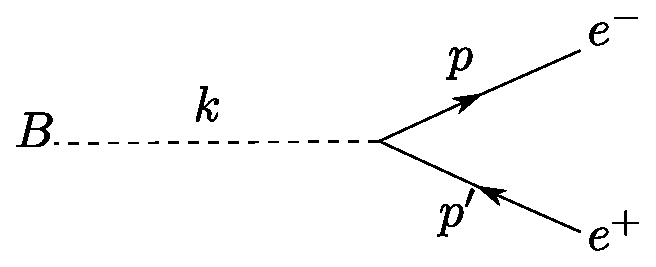
\includegraphics[scale=0.6]{Btoee} %noinstiki
  \caption{Feynman diagrams for $B\to e^+ e^-$} %noinstiki
  \label{fig:btoee} %noinstiki
\end{figure} %noinstiki
In the language of second quantization it is said that at the interaction point in Fig.~\ref{fig:btoee}, the scalar is destroyed by $\phi_+$ and one electron ($\Psi_-$) and a positron ($\bar{\Psi}_{-}$) are created.

Let us define the one--particle states as in eq.~\eqref{eq:38f}

\begin{align}
  | H(\mathbf{p})\rangle\equiv\sqrt{\frac{1}{V}}a^\dagger_{\mathbf{p}}|0\rangle 
\end{align}
For the two Weyl spinors forming a Dirac spinor we have the solutions
\begin{align}
 e_L\to \xi_{\alpha}=&\sum_s\int \frac{\operatorname{d}^3p}{(2\pi)^3\sqrt{2E_{\mathbf{p}}}} \left[ x_{\alpha}\left(s,\mathbf{p}\right) a_s e^{-i p\cdot x}+y_{\alpha}\left(s,\mathbf{p}\right) b_s^{\dagger} e^{i p\cdot x}  \right]\nonumber\\
 \left( e_L \right)^{\dagger}\to \xi_{\dot{\alpha}}^{\dagger}=&\sum_s\int \frac{\operatorname{d}^3p}{(2\pi)^3\sqrt{2E_{\mathbf{p}}}} \left[ y_{\dot{\alpha}}^{\dagger}\left(s,\mathbf{p}\right) b_s e^{-i p\cdot x}+x_{\dot{\alpha}}^{\dagger}\left(s,\mathbf{p}\right) a_s^{\dagger} e^{i p\cdot x}  \right]\nonumber\\
 \left( e_R \right)^{\dagger}\to \eta^{\alpha}=&\sum_s\int \frac{\operatorname{d}^3p}{(2\pi)^3\sqrt{2E_{\mathbf{p}}}} \left[ x^{\alpha}\left(s,\mathbf{p}\right) b_s e^{-i p\cdot x}+y^{\alpha}\left(s,\mathbf{p}\right) a_s^{\dagger} e^{i p\cdot x}  \right] \nonumber\\
  e_R\to \eta^{\dagger\dot{\alpha}}=&\sum_s\int \frac{\operatorname{d}^3p}{(2\pi)^3\sqrt{2E_{\mathbf{p}}}} \left[ y^{\dagger\dot{\alpha}}\left(s,\mathbf{p}\right) a_s e^{-i p\cdot x}+x^{\dagger\dot{\alpha}}\left(s,\mathbf{p}\right) b_s^{\dagger} e^{i p\cdot x}  \right].
\end{align}


From here we can define the one--particle states as
\begin{align}
  \label{eq:77f}
   | e_L(\mathbf{p},s)\rangle\equiv&\sqrt{\frac{1}{V}}a^\dagger_s(\mathbf{p})|0\rangle, &    | e_R(\mathbf{p},s)\rangle\equiv&\sqrt{\frac{1}{V}}a^\dagger_s(\mathbf{p})|0\rangle\nonumber\\
   | \left( e_L \right)^{\dagger}(\mathbf{p},s)\rangle\equiv&\sqrt{\frac{1}{V}}{b}^\dagger_s(\mathbf{p})|0\rangle,&
   | \left( e_R \right)^{\dagger}(\mathbf{p},s)\rangle\equiv&\sqrt{\frac{1}{V}}{b}^\dagger_s(\mathbf{p})|0\rangle\,, 
\end{align}
Using the commutation relations, our states are then normalized as
\begin{align}
\langle B(\mathbf{p})| B(\mathbf{p}')\rangle=&\frac{(2\pi)^3}{V}\delta^3(\mathbf{p}-\mathbf{p}')\nonumber\\
\langle e_{L,R}(\mathbf{p},s)| e_{L,R}(\mathbf{p}',s')\rangle=&\frac{(2\pi)^3}{V}\delta_{s s'}\delta^3(\mathbf{p}-\mathbf{p}')\nonumber\\
\langle \left( e_{L,R} \right)^{\dagger}(\mathbf{p},s)| \left( e_{L,R} \right)^{\dagger}(\mathbf{p}',s')\rangle=&\frac{(2\pi)^3}{V}\delta_{s s'}\delta^3(\mathbf{p}-\mathbf{p}')
\end{align}
As established in Sec.~\ref{sec:fock-space-real}, it is convenient to work in the discrete limit where \eqref{eq:26f}
\begin{align}
   \delta^3(\mathbf{0})=\frac{V}{(2\pi)^3}\,.
\end{align}

Now we can write down the action of various field operators on different one particles states. 
Using the Fourier decomposition  of the scalar field in eq.~\eqref{eq:37f}, and taking into account that 
$a_{\mathbf{p}}|0\rangle=0$, we have
\begin{align}
\label{eq:98f}
   \phi_+(x)|H(\mathbf{k})\rangle=&\int d^3p \frac{1}{(2\pi)^3\sqrt{2\omega_{p} }}
\widehat{a}_{p} e^{-i p\cdot x }
|H(\mathbf{k})\rangle\nonumber\\
=&\int d^3p \frac{1}{(2\pi)^3\sqrt{2\omega_{p}}}
\widehat{a}_\mathbf{p} e^{-i p\cdot x }
\frac{1}{\sqrt{V}}\, \widehat{a}^\dagger_{\mathbf{k}}|0\rangle\nonumber\\
  =&\int d^3p \frac{1}{(2\pi)^3\sqrt{2\omega_{p}V}} e^{-i p\cdot x }
\, [\widehat{a}_{\mathbf{p}},\widehat{a}^\dagger_{\mathbf{k}}]|0\rangle\,.
\end{align}
%check normalization!
By using the commutation relations in eq.~\eqref{eq:32f} we have

\begin{align}
\phi_+(x)|H(\mathbf{k})\rangle  
=&\int d^3p \frac{\delta^{(3)}(\mathbf{p}-\mathbf{k})}{\sqrt{2\omega_{p}V}}
 e^{-i p\cdot x }|0\rangle
\end{align}
\begin{align}
\phi_+(x)|H(\mathbf{k})\rangle  
=&\frac{1}{\sqrt{2\omega_{k}V}}e^{-i k\cdot x }|0\rangle
\end{align}
Similarly, we have  \emph{initial one-particles states} on left and \emph{initial one-particles states} on right
\begin{align}
  \label{eq:99f}
  \phi_+(x)|H(\mathbf{k})\rangle=&\frac{1}{\sqrt{2 \omega_k V}}e^{-i k\cdot x}|0\rangle,&
 \langle H(\mathbf{k})|\phi_-(x)=&\langle0|\frac{1}{\sqrt{2 \omega_k V}}e^{i k\cdot x}\nonumber\\
  \xi_+(x)|e_{L}(\mathbf{p},s)\rangle=&\frac{1}{\sqrt{2 E_p V}}x(s,\mathbf{p})e^{-i p\cdot x}|0\rangle,&
  \langle e_{L}(\mathbf{p},s)|\xi_-^{\dagger}(x)=&\langle 0|\frac{1}{\sqrt{2 E_p V}}x^{\dagger}(s,\mathbf{p})e^{i p\cdot x}\nonumber\\
  \eta_+(x)|\left( e_R \right)^{\dagger}(\mathbf{p},s)\rangle=&\frac{1}{\sqrt{2 E_{p} V}}x(s,\mathbf{p})e^{-i p\cdot x}|0\rangle,&
  \langle \left( e_R \right)^{\dagger}(\mathbf{p},s)|\eta^{\dagger}_-(x)=&\langle 0|\frac{1}{\sqrt{2 E_{p} V}}x(s,\mathbf{p})e^{i p\cdot x} \nonumber\\
  \xi_+^{\dagger}(x)|\left( e_{L} \right)^{\dagger}(\mathbf{p},s)\rangle=&\frac{1}{\sqrt{2 E_p V}}y^{\dagger}(s,\mathbf{p})e^{-i p\cdot x}|0\rangle,&
  \langle\left( e_{L} \right)^{\dagger}(\mathbf{p},s)|\xi_-(x)=&\langle 0| \frac{1}{\sqrt{2 E_p V}}y(s,\mathbf{p})e^{i p\cdot x}\nonumber\\
  \eta_+^{\dagger}(x)|e_R (\mathbf{p},s)\rangle=&\frac{1}{\sqrt{2 E_{p} V}}y^{\dagger}(s,\mathbf{p})e^{-i p\cdot x}|0\rangle,&
  \langle e_R(\mathbf{p},s)|\eta_-(x)=&\langle 0|\frac{1}{\sqrt{2 E_{p'} V}}y(s,\mathbf{p})e^{i p\cdot x}
 \,.
\end{align}
where $\omega_k$ and $E_p$ represent the energies of the scalar and the electron for the 3-momenta in the subscripts.

In the lowest order the only term which contributes to the matrix element is the term shown in Eq.~\eqref{eq:97f}.
The matrix element at first order in eq.~\eqref{eq:S1}, between the initial and the final state is then
\begin{align}
  S_{fi}^{(1)}=-i y \int \operatorname{d}^4x \left[ \left\langle e_L(p)\left( e_R \right)^{\dagger}(p') \left|\xi_-^{\dagger}\eta_-^{\dagger} \phi_{+}  \right|H(\mathbf{k}),0,0 \right\rangle
+\left\langle \left( e_L \right)^{\dagger}(p) e_R (p') \right|\xi_-\eta_- \phi_{+}  \left|H(\mathbf{k}),0,0 \right\rangle \right] 
\end{align}
Using Eqs.~\eqref{eq:99f}  we obtain
\begin{align}
  S_{fi}^{(1)}=&(-i y) \left[ x^{\dagger}_{\dot{\alpha}}{x^{\dagger}}^{\dot{\alpha}}+y^{\alpha}y_{\alpha} \right]
\int d^4x\,e^{i(p+p'-k)\cdot x}\frac{1}{\sqrt{2\omega_k V}}\frac{1}{\sqrt{2E_p V}}\frac{1}{\sqrt{2E_{p'} V}}\,.
\end{align}
Since
\begin{align}
  \int d^4x\,e^{i(p+p'-k)\cdot x}=(2\pi)^4\delta^4(k-p-p')\,,
\end{align}
we obtain
\begin{align}
  S_{fi}^{(1)}=&\left[\frac{1}{\sqrt{2\omega_k V}}\frac{1}{\sqrt{2E_p V}}\frac{1}{\sqrt{2E_{p'} V}}\right]
(2\pi)^4\delta^4(k-p-p')(-i y)\left[ x^{\dagger}_{\dot{\alpha}}{x^{\dagger}}^{\dot{\alpha}}+y^{\alpha}y_{\alpha} \right].
\end{align}
Comparing with Eq.~\eqref{eq:RMfi} we have therefore that the relativistic matrix element is
\begin{align}
  i\mathcal{M}_{fi}=-i y\left[ x^{\dagger}_{\dot{\alpha}}{x^{\dagger}}^{\dot{\alpha}}+y^{\alpha}y_{\alpha} \right].
\end{align}
Check the specific calculation in~\ref{Dreiner:2008tw}

\subsection{Yukawa interaction for Weyl fermions}
Left-handed fermion:
\begin{align}
%e_L -> e_L^- + (e_R^+)^{\dagger}
e_L\to  \xi_{\alpha}=&\int \frac{d^3 p}{(2\pi)^3\sqrt{2E_{\mathbf{p}}}} \left[ x_{\alpha}(\mathbf{p},s)a(\mathbf{p},s)\operatorname{e}^{-i p\cdot x}+y_{\alpha}(\mathbf{p},s)a^{\dagger}(\mathbf{p},s)\operatorname{e}^{i p\cdot x} \right] \nonumber\\
%(e_L)^{\dagger} -> e_R^+ + (e_L^-)^{\dagger}
\left( e_L \right)^{\dagger}\to  \xi_{\dot{\alpha}}^{\dagger}=&\int \frac{d^3 p}{(2\pi)^3\sqrt{2E_{\mathbf{p}}}} \left[y_{\dot{\alpha}}^{\dagger}(\mathbf{p},s)a(\mathbf{p},s)\operatorname{e}^{-i p\cdot x}+ x_{\dot{\alpha}}^{\dagger}(\mathbf{p},s)a^{\dagger}(\mathbf{p},s)\operatorname{e}^{i p\cdot x}\right] .
\end{align}

Right-handed fermion 
\begin{align}
%e_R -> e_R^- + (e_L^+)^{\dagger}
e_R\to  \eta^{\dagger\dot{\alpha}}=&\int \frac{d^3 p}{(2\pi)^3\sqrt{2E_{\mathbf{p}}}} \left[y^{\prime\dot{\alpha}\dagger}(\mathbf{p},s)b(\mathbf{p},s)\operatorname{e}^{-i p\cdot x}+ x^{\prime\dot{\alpha}\dagger}(\mathbf{p},s)b^{\dagger}(\mathbf{p},s)\operatorname{e}^{i p\cdot x} \right] .
 \nonumber\\
%(e_R)^{\dagger} -> e_L^+ + (e_R^-)^{\dagger}
\left( e_R \right)^{\dagger}\to  \eta^{\alpha}=&\int \frac{d^3 p}{(2\pi)^3\sqrt{2E_{\mathbf{p}}}} \left[ x^{\prime\alpha}(\mathbf{p},s)b(\mathbf{p},s)\operatorname{e}^{-i p\cdot x}+y^{\prime\,\alpha}(\mathbf{p},s)b^{\dagger}(\mathbf{p},s)\operatorname{e}^{i p\cdot x} \right]
\end{align}
\begin{align}
 \xi_{+} | e^{-}_{L}\rangle =& x a a^{\dagger} |0\rangle \nonumber\\
 \eta_{+} | \left( e^{-}_{R} \right)^{\dagger}\rangle =& x' b b^{\dagger} |0\rangle \nonumber\\
 \xi_{+} |  \left( e^{-}_{L} \right)^{\dagger} \rangle =& y^{\dagger} a a^{\dagger} |0\rangle \nonumber\\
 \eta_{+} | e^{-}_{R} \rangle =& y^{\prime \dagger} b b^{\dagger} |0\rangle
\end{align}
After some calcultations ...

From the cojugate relations, e.g $\langle e_L^- |\xi_-=\langle 0|x^{\dagger}...$, etc
\begin{align}
  \mathcal{M}_1 =& x^{\dagger} x^{\prime \dagger} &\mathcal{M}_2=& y y'
\end{align}
\section{Wick Theorem}
\label{sec:wick-theorem}

\subsection{Basics concepts}
Return back to  the interpretation of interaction in terms of one exchanged particle, as illustrated again in Fig.~\ref{fig:qedrepulsionx1x2}
\begin{figure}
  \centering
  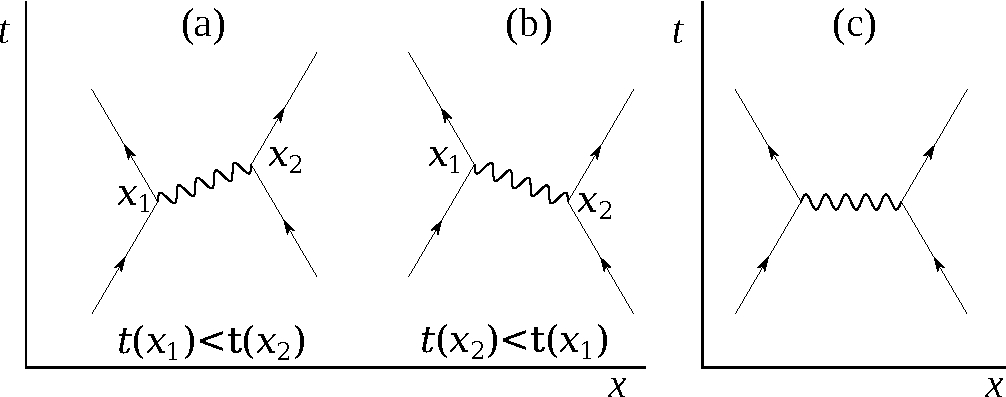
\includegraphics{qedrepulsionx1x2}
  \caption{Electromagnetic repulsion. The diagrams (a) and (b) are summarized in the diagram (c)}
  \label{fig:qedrepulsionx1x2}
\end{figure}


From \cite{Lahiri:2005sm}. The normal ordering procedure involved putting all the annihilation operators to the right of all creation operators so that it annihilates the vacuum. But the time ordering raises complications because in it all operators at earlier times must be further to the right. So creation operators at later times would be to the right of annihilation operators at later times, contrary to what we need for normal ordering. The advantage of normal ordered products is that their expectation values vanish in the vacuum. 

If $H_I$ contains an even number of fermion factors, we can use the time--ordered product $\operatorname{T}\{\ldots\}$ of $n$ factors to write this expression in the equivalent form. For $S^{(2)}$ we have for example
\begin{align}
 \int_{-\infty}^\infty dt_1 \int_{-\infty}^{\infty}d t_2 \operatorname{T}\{H_I(t_1)H_I(t_2)\}=&
\int_{-\infty}^\infty dt_1\int_{-\infty}^{\infty}d t_2 \theta(t_2-t_1)H_I(t_2)H_I(t_1) \nonumber\\
&+\int_{-\infty}^\infty dt_1\int_{-\infty}^{\infty}d t_2 \theta(t_1-t_2)H_I(t_1)H_I(t_2)
 \end{align}
where, for $t_2$ and $t_1$ fixed respectively
 \begin{align}
   \theta(t_2-t_1)=&
   \begin{cases}
    0\, &    t_1> t_2\\
    1\, &    t_1< t_2\\
   \end{cases},&   \theta(t_1-t_2)=&
   \begin{cases}
    0\, &    t_2> t_1\\
    1\, &    t_2< t_1\\
   \end{cases}\,.
 \end{align}
In this way.
\begin{align}
 \int_{-\infty}^\infty dt_1 \int_{-\infty}^{\infty}d t_2 \operatorname{T}\{H_I(t_1)H_I(t_2)\}=&
\int_{-\infty}^\infty dt_2\int_{-\infty}^{t_2}d t_1 \theta(t_2-t_1)H_I(t_2)H_I(t_1)\nonumber\\
&+\cancel{\int_{-\infty}^\infty dt_2\int_{t_2}^{t_1}d t_1 \theta(t_2-t_1)H_I(t_2)H_I(t_1)} \nonumber\\
&+\int_{-\infty}^\infty dt_1\int_{-\infty}^{t_{1}}d t_2 \theta(t_1-t_2)H_I(t_1)H_I(t_2) \nonumber\\
&+\cancel{\int_{-\infty}^\infty dt_1\int_{t_1}^{t_2}d t_2 \theta(t_1-t_2)H_I(t_1)H_I(t_2)}\,.
\end{align}
The integral in $dt_1'$ is for $t_1>t_2$, with $t_2$ fixed, so that $\theta(t_2-t_1')=0$ for $t_1'>t_2$. Similarly,
The integral in $dt_2'$ is for $t_2>t_1$, with $t_1$ fixed, so that $\theta(t_1-t_2')=0$ for $t_2'>t_1$. Therefore,
\begin{align}
   \int_{-\infty}^\infty dt_1 \int_{-\infty}^{\infty}d t_2 \operatorname{T}\{H_I(t_1)H_I(t_2)\}=&
\int_{-\infty}^\infty dt_2\int_{-\infty}^{t_2}d t_1 H_I(t_2)H_I(t_1)
+\int_{-\infty}^\infty dt_1\int_{-\infty}^{t_{1}}d t_2 H_I(t_1)H_I(t_2)\nonumber\\
=&
\int_{-\infty}^\infty dt_1\int_{-\infty}^{t_1}d t_2 H_I(t_1)H_I(t_2)
+\int_{-\infty}^\infty dt_1\int_{-\infty}^{t_{1}}d t_2 H_I(t_1)H_I(t_2) \nonumber\\
=&
2\int_{-\infty}^\infty dt_1\int_{-\infty}^{t_1}d t_2 H_I(t_1)H_I(t_2)\,.
\end{align}
In terms of the ordering operator all the integrals are between $-\infty$ to $\infty$:
\begin{align}
   S=&1+\sum_{n=1}^\infty\frac{(-i)^n}{n!}\int_{-\infty}^{\infty}d t_1\,\int_{-\infty}^{\infty} d t_2\ldots\int_{-\infty}^{\infty}d t_n\,\operatorname{T}\{{H}_I(t_1){H}_I(t_2)\ldots{H}_I(t_n)\}\,, 
\end{align}
In terms of the Hamiltonian density, we have
\begin{align}
  S=1+\sum_{n=1}^\infty\frac{(-i)^n}{n!}\int\cdots\int d^4x_1 d^4x_2\ldots d^4x_n\,\operatorname{T}\{\mathcal{H}_I(x_1)\mathcal{H}_I(x_2)\ldots\mathcal{H}_I(x_n)\}\,, 
\end{align}
In the above perturbation formalism the states $|i\rangle$ and $|f\rangle$ are, as usual, eigenstates of the unperturbed free-field Hamiltonian $H_0$. As such can be introduced inside the integrals
\begin{align}
  S_{f i}=&\langle f|S|i\rangle\nonumber\\
  =&1+\sum_{n=1}^\infty\frac{(-i)^n}{n!}\int\cdots\int d^4x_1 d^4x_2\ldots d^4x_n\,\langle f|\operatorname{T}\{\mathcal{H}_I(x_1)\mathcal{H}_I(x_2)\ldots\mathcal{H}_I(x_n)\}|i\rangle\,.
\end{align}


For example, at first order
\begin{align}
  \label{eq:96f}
  S_{fi}^{(1)}=&\langle f|S^{(1)}|i\rangle\nonumber\\
  =&\langle f|-i\int d^4x_1\,\operatorname{T}\{\mathcal{H}_I(x_1)\}|i\rangle\nonumber\\
  =&-i\int d^4x_1\,\langle f|:\mathcal{H}_I(x_1):|i\rangle\,.
\end{align}
In order to evaluate this integrals we need to write the time ordered product in terms of the fields. This can done by induction. We start by considering the simple no trivial case with two scalar fields
%ver cuaderno de perrito


\subsection{Scalar propagator}

With
\begin{align}
  \bcontraction{\,}{\phi}{(x_1)}{\phi}
\,\phi(x_1)\phi(x_2)\equiv \left\langle 0 |   T\{\phi(x_1)\phi(x_2)\} | 0 \right\rangle
\end{align}




The Wick contraction can be written as:
\begin{align}
\label{eq:77f}
  \bcontraction{\,}{\phi}{(x_1)}{\phi}
\,\phi(x_1)\phi(x_2)=&\langle0|T\{\phi(x_1)\phi(x_2)\}|0\rangle\nonumber\\
=&i\Delta_F(x_1-x_2)
\end{align}
since
\begin{align}
  \phi(x)=\phi_+(x)+\phi_-(x)\,,
\end{align}
\begin{align}
T\left[\phi(x_1),\phi(x_2)\right]=\theta(t_1-t_2)\phi(x_1)\phi(x_2)+\theta(t_2-t_1)\phi(x_2)\phi(x_1)
\end{align}
\begin{align}
    \langle0|T\left[\phi(x_1),\phi(x_2)\right]|0\rangle=&\theta(t_1-t_2)\langle0|\phi(x_1)\phi(x_2)+\theta(t_2-t_1)\langle0|\phi(x_2)\phi(x_1)|0\rangle\nonumber\\
   =&\theta(t_1-t_2)\langle0|\phi_+(x_1)\phi_-(x_2)+\theta(t_2-t_1)\langle0|\phi_+(x_2)\phi_-(x_1)|0\rangle\nonumber\\
     =&\langle0|\theta(t_1-t_2)\phi(x_1)_+\phi_-(x_2)+\theta(t_2-t_1)\langle0|\phi_+(x_2)\phi_-(x_1)|0\rangle
\end{align}

with
\begin{align}
    \phi_+(x)=&\int d^3p \frac{1}{(2\pi)^3\sqrt{2\omega_{p} }}
\widehat{a}_{p} e^{-i p\cdot x }&
    \phi_-(x)=&\int d^3p \frac{1}{(2\pi)^3\sqrt{2\omega_{p} }}
\widehat{a}_{p}^\dagger e^{i p\cdot x }\,,
\end{align}
we have
\begin{align}
  \langle0|T(\phi(x_1)\phi(x_2))|0\rangle
=&\theta(t_1-t_2)\langle0|\int\frac{d^3p_1}{(2\pi)^3\sqrt{2E_{p_1}}}\hat{a}_{p_1}e^{-i p_1\cdot x_1}
\int\frac{d^3p_2}{(2\pi)^3\sqrt{2E_{p_2}}}\hat{a}_{p_2}^\dagger e^{-i p_2\cdot x_2}|0\rangle\nonumber\\
&+\theta(t_2-t_1)\langle0|\int\frac{d^3p_2}{(2\pi)^3\sqrt{2E_{p_2}}}\hat{a}_{p_2}e^{-i p_2\cdot x_2}
\int\frac{d^3p_1}{(2\pi)^3\sqrt{2E_{p_1}}}\hat{a}_{p_1}^\dagger e^{-i p_1\cdot x_1}|0\rangle\nonumber\\
=&\theta(t_1-t_2)\int\int\frac{d^3p_1d^3p_2}{(2\pi)^6\sqrt{2E_{p_1}}\sqrt{2E_{p_2}}}e^{-i p_1\cdot x_1}e^{-i p_2\cdot x_2}
\langle0|\hat{a}_{p_1}\hat{a}_{p_2}^\dagger|0\rangle\nonumber\\
&+\theta(t_2-t_1)\int\int\frac{d^3p_2d^3p_1}{(2\pi)^6\sqrt{2E_{p_2}}\sqrt{2E_{p_1}}}e^{-i p_2\cdot x_2}e^{-i p_1\cdot x_1}
\langle0|\hat{a}_{p_2}\hat{a}_{p_1}^\dagger|0\rangle\nonumber\\
\end{align}

\begin{align}
=&\theta(t_1-t_2)\int\int\frac{d^3p_1d^3p_2}{(2\pi)^6\sqrt{2E_{p_1}}\sqrt{2E_{p_2}}}e^{-i p_1\cdot x_1}e^{-i p_2\cdot x_2}
\langle0|\hat{a}_{p_1}\hat{a}_{p_2}^\dagger|0\rangle\nonumber\\
&+\theta(t_2-t_1)\int\int\frac{d^3p_2d^3p_1}{(2\pi)^6\sqrt{2E_{p_2}}\sqrt{2E_{p_1}}}e^{-i p_2\cdot x_2}e^{-i p_1\cdot x_1}
\langle0|\hat{a}_{p_2}\hat{a}_{p_1}^\dagger|0\rangle\nonumber\\
\end{align}

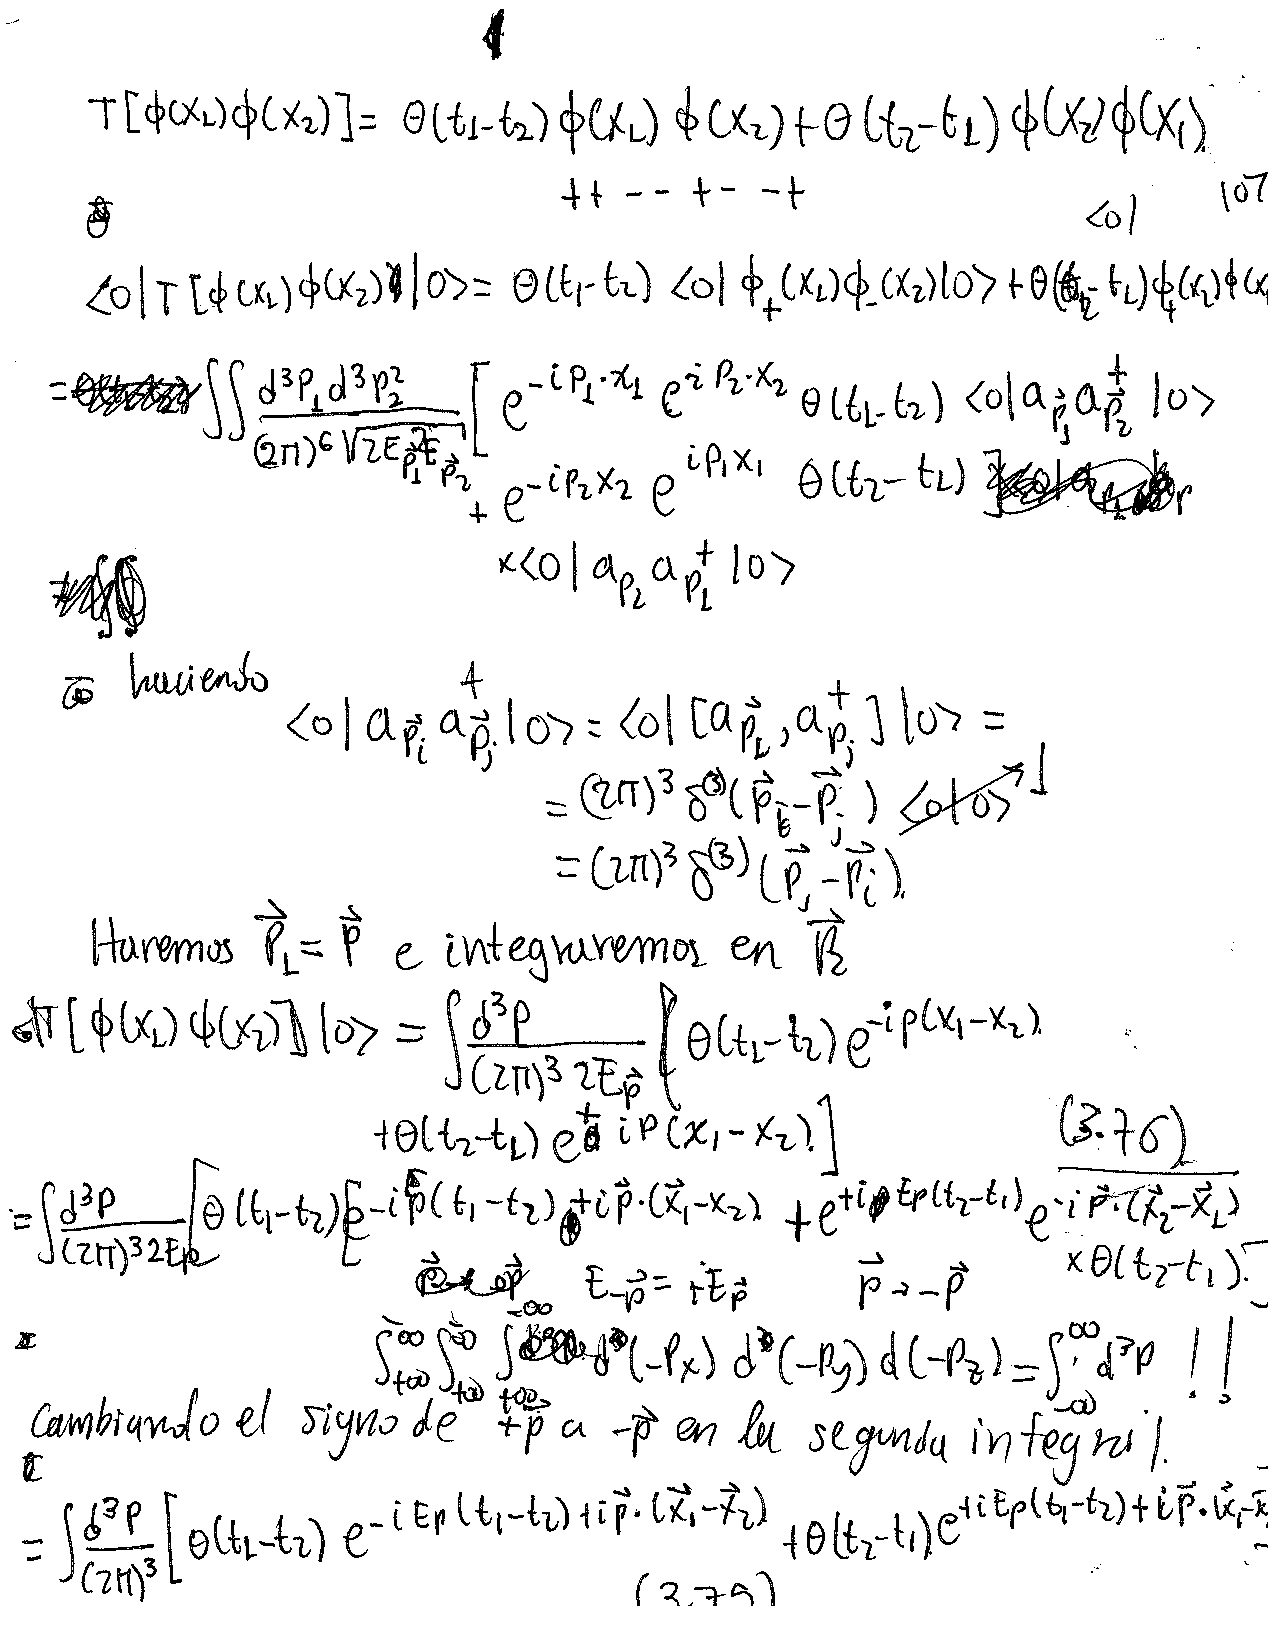
\includepdf[pages=-]{propagator.pdf}  

\subsection{Wick theorem}
\begin{align}
  T\{\phi(x_1)\phi(x_2)\}=:\phi(x_1)\phi(x_2):+\bcontraction{\,}{\phi}{(x_1)}{\phi}
\,\phi(x_1)\phi(x_2)
\end{align}
The same expression can be obtained for fermions.

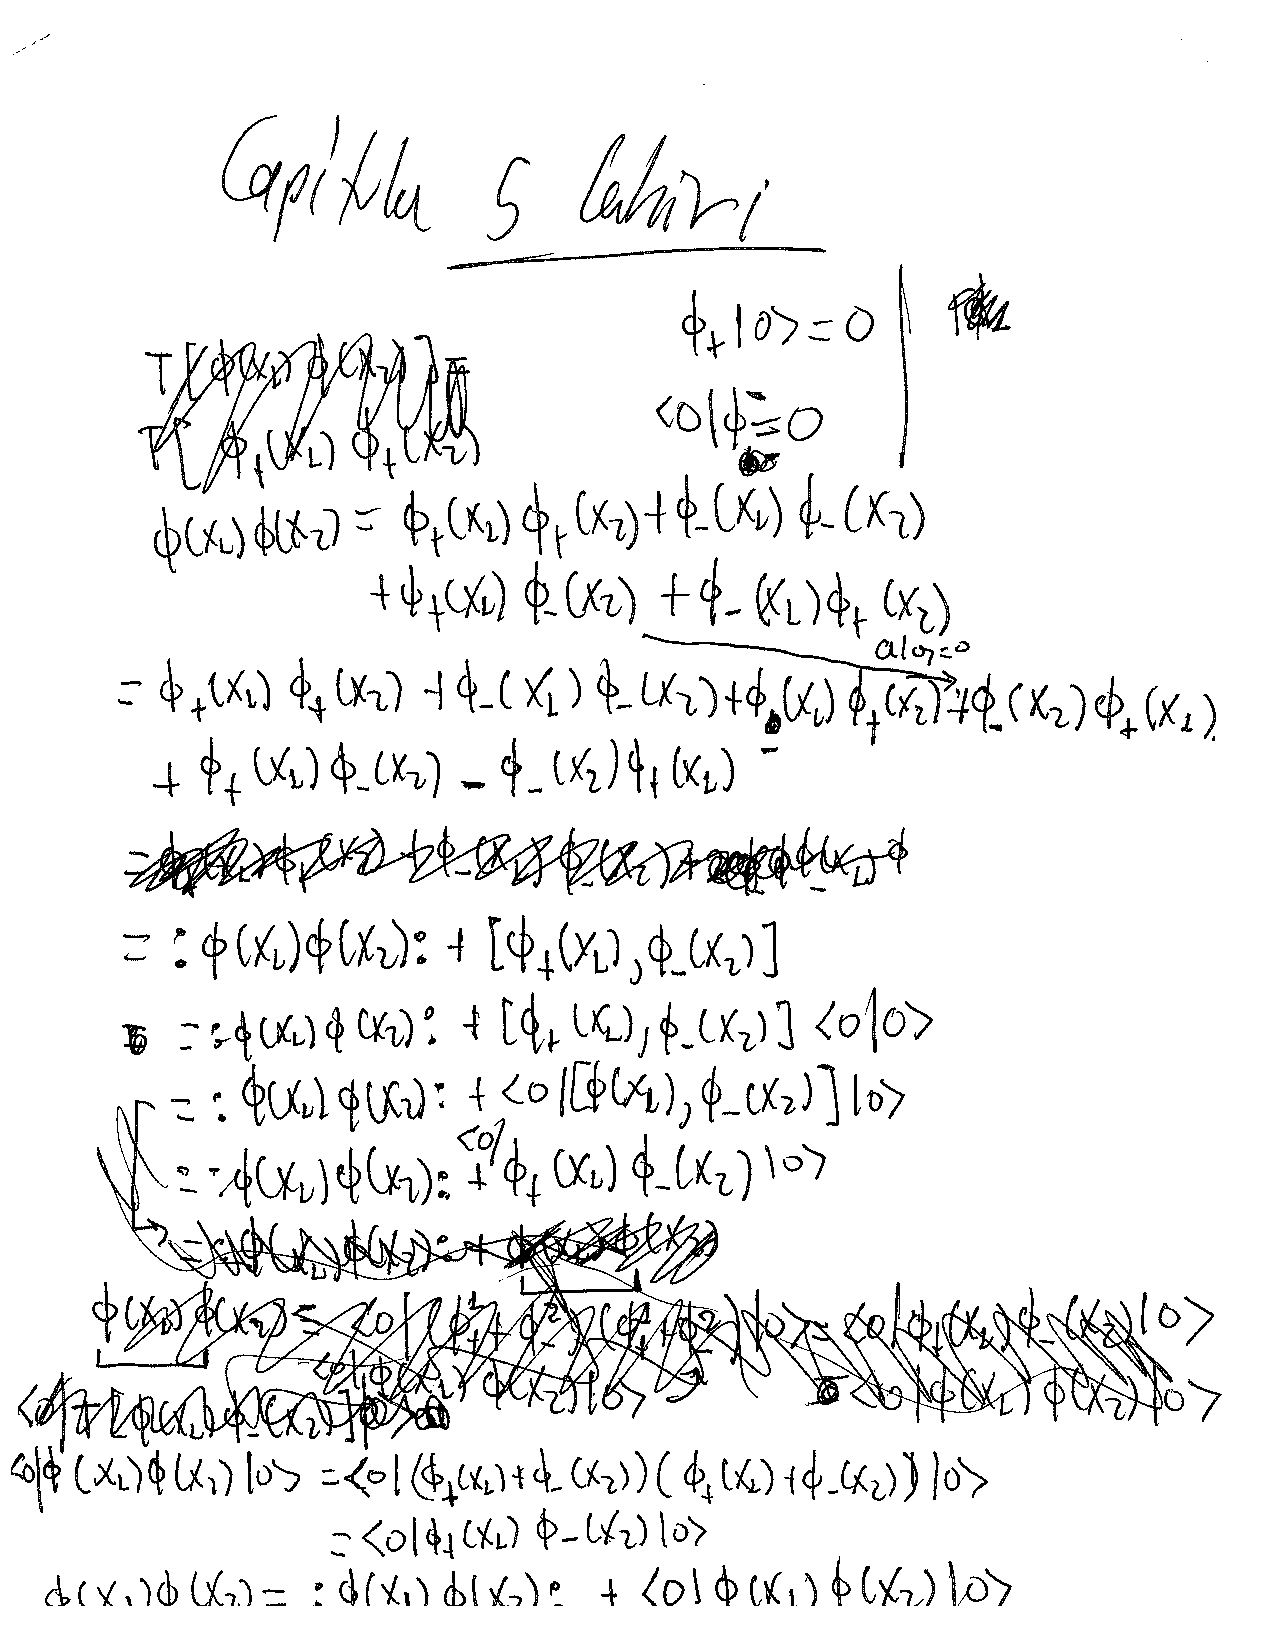
\includepdf[pages=-]{wick.pdf}  


 Generalizing  the results for $n$ scalar or fermion fields, but with an even number of fermions fields, we have the Wick theorem
\begin{align}
  T\{\Phi(x_1)\Phi(x_2)\Phi(x_3)\cdots\Phi(x_n) \}
=&:\Phi(x_1)\Phi(x_2)\Phi(x_3)\cdots\Phi(x_n):+\nonumber\\
&+\bcontraction{\,}{\Phi}{(x_1)}{\Phi}\,\Phi(x_1)\Phi(x_2):\Phi(x_3)\cdots\Phi(x_n):\nonumber\\
&+:\Phi(x_1)\bcontraction{\,}{\Phi}{(x_2)}{\Phi}\,\Phi(x_2)\Phi(x_3)\cdots\Phi(x_n):+\cdots  \nonumber\\
=&:\Phi(x_1)\Phi(x_2)\Phi(x_3)\cdots\Phi(x_n):+\nonumber\\
&+\left[:\bcontraction{\,}{\Phi}{(x_1)}{\Phi}\,\Phi(x_1)\Phi(x_2)\Phi(x_3)\cdots\Phi(x_n): +\text{perm} \right]\nonumber\\
&+\left[  :\bcontraction{\,}{\Phi}{(x_1)}{\Phi}\,\Phi(x_1)\Phi(x_2) \bcontraction{\,}{\Phi}{(x_3)}{\Phi}\,\Phi(x_3)\Phi(x_4)\Phi(x_5)\cdots\Phi(x_n): +\text{perm}  \right] \nonumber\\
&+\cdots \nonumber\\
\end{align}
For details of the full result see for example \cite{Lahiri:2005sm}.


\section{Scattering}
\label{sec:scattering}
From the previous calculation we have
\begin{align}
S^{(n)}=  \frac{(-i)^n}{n!}\int\cdots\int d^4x_1 d^4x_2\ldots d^4x_n\,\operatorname{T}\{\mathcal{H}_I(x_1)\mathcal{H}_I(x_2)\ldots\mathcal{H}_I(x_n)\}\,.
\end{align}
The relevant term for the scattering
\begin{align}
  e^{-}_L(p_1)+e_L^{-}(p_2)\to   e_R^{-}(p_1')+e_R^{-}(p_2')
\end{align}
As alwayas we use the left-handed Weyl spinors
\begin{align}
  e_L\to &\xi_{\alpha} &   \left( e_R \right)^{\dagger}\to &\eta^{\alpha}\,,
\end{align}
with Yukawa Lagrangian
\begin{align}
  \mathcal{L}_y=& y \left(e_R\right)^{\dagger} e_L h^0 +y \left(e_L\right)^{\dagger} e_R h^0 \nonumber\\
               =& y \eta^{\alpha} \xi_{\alpha}h^0 + y \eta^{\dagger\dot{\alpha}} \xi_{\dot{\alpha}}^{\dagger}h^0\,. 
\end{align}


is
\begin{align}
S^{(2)}=&  \frac{(-i)^2}{2!}\int\int d^4x_1 d^4x_2\,\operatorname{T}\{\mathcal{H}_I(x_1)\mathcal{H}_I(x_2)\}\nonumber\\
=&  \frac{(-iy)^2}{2!}\int\int d^4x_1 d^4x_2\,\operatorname{T}\{\left( \eta^{\alpha} \xi_{\alpha}h^0 \right)_{x_1} \left( \eta^{\alpha} \xi_{\alpha}h^0 \right)_{x_2}\}\nonumber\\
=& 
 \frac{(-iy)^2}{2!}\int\int d^4x_1 d^4x_2\,:\left( \eta^{\alpha} \xi_{\alpha}h^0 \right)_{x_1} \left( \eta^{\alpha} \xi_{\alpha}h^0 \right)_{x_2}:
 \frac{(-iy)^2}{2!}\int\int d^4x_1 d^4x_2\,:( \eta^{\alpha} 
\bcontraction{\xi_{\alpha}}{\phi}{)_{x_1}(\eta^{\alpha} \xi_{\alpha}}{h^0}
\xi_{\alpha} h^0)_{x_1}(\eta^{\alpha} \xi_{\alpha}h^0 
)_{x_2}:+\cdots
\end{align}
The first term corresponds to two  disconnected Feynman diagrams that does not contribute to the $S$--matrix. For the process at hand, we want terms where four fermionic operators are not contracted, corresponding to the particles in the initial and final states. The second term in the previous expansion of the Wick theorem is the only satisfying this requirement. In this way
\begin{align}
  S^{(2)}(e^+ e^-\to e^+e^-)=&\frac{(-iy)^2}{2!}\int\int d^4x_1 d^4x_2
\bcontraction{\,}{\phi}{(x_1)}{\phi}
\,\phi(x_1)\phi(x_2):(\eta^{\alpha} \xi_{\alpha})_{x_1}(\eta^{\beta} \xi_{\beta})_{x_2}:
\end{align}

On the other hand 
\begin{align}
\label{eq:156f}
  :(\eta^{\alpha} \xi_{\alpha})_{x_1}(\eta^{\beta} \xi_{\beta})_{x_2}:=&
:\eta^{\alpha}(x_1) \xi_{\alpha}(x_1) \eta^{\beta}(x_2) \xi_{\beta}(x_2):\,.
\end{align}

%\left[\right]
%\left(\right)



The specific calculation by the scattering mediated by the Higgs is 
\begin{align}
  S_{fi}=&\frac{\left( -iy \right)^{2}}{2!}\sum_{\text{spins}}\int\int \operatorname{d}^4x_1 \operatorname{d}^4x_2
\bcontraction{\,}{\phi}{(x_1)}{\phi}\,\phi(x_1)\phi(x_2) \nonumber\\
&\left\langle e_R\left(\mathbf{p}'_1\right), e_R \left(\mathbf{p}'_2\right) \right|
  :\eta^{\alpha}(x_1) \eta^{\beta}(x_2)\xi_{\beta}(x_2) \xi_{\alpha}(x_1):
 \left| e_L \left(\mathbf{p}_1\right), e_L\left(\mathbf{p}_2\right) \right\rangle. \nonumber\\
  =&\frac{\left( -iy \right)^{2}}{2!}\sum_{\text{spins}}\int\int \operatorname{d}^4x_1 \operatorname{d}^4x_2
\,i\Delta_F(x_1-x_2) \nonumber\\
&\left\langle e_R\left(\mathbf{p}'_1\right), e_R \left(\mathbf{p}'_2\right) \right|
  \eta^{\alpha}_{-}(x_1) \eta^{\beta}_{-}(x_2)\xi_{\beta +}(x_2) \xi_{\alpha +}(x_1)
 \left| e_L \left(\mathbf{p}_1\right), e_L\left(\mathbf{p}_2\right) \right\rangle. \nonumber\\
  =&\frac{\left( -iy \right)^{2}}{2!}\sum_{\text{spins}}\int\int \operatorname{d}^4x_1 \operatorname{d}^4x_2
\int\frac{d^4q}{(2\pi)^4}\,i\Delta_F(q)\operatorname{e}^{i q\cdot(x_1-x_2)} \nonumber\\
&\left\langle e_R\left(\mathbf{p}'_1\right), e_R \left(\mathbf{p}'_2\right) \right|
  \eta^{\alpha}_{-}(x_1) \eta^{\beta}_{-}(x_2)\xi_{\beta +}(x_2) \xi_{\alpha +}(x_1)
 \left| e_L \left(\mathbf{p}_1\right), e_L\left(\mathbf{p}_2\right) \right\rangle. 
\end{align}
In the following, to avoid clutter in the expressions we ignore the spin part during the intemediate calculations. 
The two particle Fock state is, after proper normalization
\begin{align}
  |e_L(\mathbf{p}_2)e_L(\mathbf{p}_1)\rangle=&\frac{1}{\sqrt{V^2}}a_{s_1}^\dagger(\mathbf{p}_1)a_{s_2}^\dagger(\mathbf{p}_2)|0\rangle
\end{align}
Therefore %recalculate
\begin{align}
  \xi^\alpha_+(x_1)\xi^\beta_+(x_2)|e_L^-(\mathbf{p}_2)e_L^-(\mathbf{p}_1)\rangle=&
\int\frac{d^3k}{(2\pi)^3\sqrt{2E_k V}}\int\frac{d^3k'}{(2\pi)^3\sqrt{2E_{k'}V}}
x^\alpha(s,\mathbf{k})x^\beta(s',\mathbf{k}')\operatorname{e}^{-i k\cdot x_1}\operatorname{e}^{-i k'\cdot x_2}\nonumber\\
&\times a_s(\mathbf{k})a_{s'}(\mathbf{k}')a_{s_1}^\dagger(\mathbf{p}_1)a_{s_2}^\dagger(\mathbf{p}_2)|0\rangle \nonumber\\
=&
\int\frac{d^3k'}{(2\pi)^3\sqrt{2E_k V}}\int\frac{d^3k}{(2\pi)^3\sqrt{2E_{k'}V}}
x^\alpha(s,\mathbf{k})x^\beta(s',\mathbf{k}')\operatorname{e}^{-i k\cdot x_1}\operatorname{e}^{-i k'\cdot x_2}\nonumber\\
&\times \left[ a_s(\mathbf{k})a_{s'}(\mathbf{k}')a_{s_1}^\dagger(\mathbf{p}_1)a_{s_2}^\dagger(\mathbf{p}_2) - a_{s_1}^\dagger(\mathbf{p}_1)a_{s_2}^\dagger(\mathbf{p}_2) a_s(\mathbf{k})a_{s'}(\mathbf{k}') \right]|0\rangle \nonumber\\
=&
\int\frac{d^3k}{(2\pi)^3\sqrt{2E_k V}}\int\frac{d^3k'}{(2\pi)^3\sqrt{2E_{k'}V}}
x^\alpha(s,\mathbf{k})x^\beta(s',\mathbf{k}')\operatorname{e}^{-i k\cdot x_1}\operatorname{e}^{-i k'\cdot x_2}\nonumber\\
&\times \left[ a_s(\mathbf{k})a_{s'}(\mathbf{k}'),a_{s_1}^\dagger(\mathbf{p}_1)a_{s_2}^\dagger(\mathbf{p}_2)\right]|0\rangle.
\end{align}
By using the identity
\begin{align}
  [AB,CD]=A[B,C]D - [A,C]BD
+CA[B, D] - C[A, D]B\,,
\end{align}
\begin{align}
   \left[ a_s(\mathbf{k})a_{s'}(\mathbf{k}'),a_{s_1}^\dagger(\mathbf{p}_1)a_{s_2}^\dagger(\mathbf{p}_2)\right]=&
 a_s(\mathbf{k})\left[ a_{s'}(\mathbf{k}'),a_{s_1}^\dagger(\mathbf{p}_1)\right]a_{s_2}^\dagger(\mathbf{p}_2)
-
 \left[ a_s(\mathbf{k}),a_{s_1}^\dagger(\mathbf{p}_1)\right]a_{s'}(\mathbf{k}')a_{s_2}^\dagger(\mathbf{p}_2) \nonumber\\
& 
+a_{s_1}^\dagger(\mathbf{p}_1)a_s(\mathbf{k})\left[ a_{s'}(\mathbf{k}'),a_{s_2}^\dagger(\mathbf{p}_2)\right]
-
a_{s_1}^\dagger(\mathbf{p}_1) \left[ a_s(\mathbf{k}),a_{s_2}^\dagger(\mathbf{p}_2)\right]a_{s'}(\mathbf{k}') \nonumber\\
=&
 \left[ a_{s'}(\mathbf{k}'),a_{s_1}^\dagger(\mathbf{p}_1)\right]a_s(\mathbf{k})a_{s_2}^\dagger(\mathbf{p}_2)
-
 \left[ a_s(\mathbf{k}),a_{s_1}^\dagger(\mathbf{p}_1)\right]a_{s'}(\mathbf{k}')a_{s_2}^\dagger(\mathbf{p}_2) \nonumber\\
& 
+\left[ a_{s'}(\mathbf{k}'),a_{s_2}^\dagger(\mathbf{p}_2)\right]a_{s_1}^\dagger(\mathbf{p}_1)a_s(\mathbf{k})
-
 \left[ a_s(\mathbf{k}),a_{s_2}^\dagger(\mathbf{p}_2)\right]a_{s_1}^\dagger(\mathbf{p}_1)a_{s'}(\mathbf{k}')
\end{align}
Therefore,
\begin{align}
&\left[ a_s(\mathbf{k})a_{s'}(\mathbf{k}'),a_{s_1}^\dagger(\mathbf{p}_1)a_{s_2}^\dagger(\mathbf{p}_2)\right] |0\rangle \nonumber\\
&\qquad=\left[ a_{s'}(\mathbf{k}'),a_{s_1}^\dagger(\mathbf{p}_1)\right]a_s(\mathbf{k})a_{s_2}^\dagger(\mathbf{p}_2) |0\rangle
-
 \left[ a_s(\mathbf{k}),a_{s_1}^\dagger(\mathbf{p}_1)\right]a_{s'}(\mathbf{k}')a_{s_2}^\dagger(\mathbf{p}_2) |0\rangle \nonumber\\
&\qquad=\left[ a_{s'}(\mathbf{k}'),a_{s_1}^\dagger(\mathbf{p}_1)\right] \left[a_s(\mathbf{k}),a_{s_2}^\dagger(\mathbf{p}_2)  \right] |0\rangle-
  \left[ a_s(\mathbf{k}),a_{s_1}^\dagger(\mathbf{p}_1)\right] \left[ a_{s'}(\mathbf{k}'),a_{s_2}^\dagger(\mathbf{p}_2)  \right] |0\rangle \nonumber\\
&\qquad= (2\pi)^6 \left[ \delta^{(3)}(\mathbf{k}'-\mathbf{p}_1)\delta^{(3)}(\mathbf{k}-\mathbf{p}_2) 
    -\delta^{(3)}(\mathbf{k}-\mathbf{p}_1)\delta^{(3)}(\mathbf{k}'-\mathbf{p}_2) \right]|0\rangle
\end{align}


\begin{align}
\label{eq:belel}
  \xi^\alpha_+(x_1)&\xi^\beta_+(x_2)|e_L^-(\mathbf{p}_2)e_L^-(\mathbf{p}_1)\rangle
 \nonumber\\
&=\frac{1 }{\sqrt{2 E_1V}\sqrt{2 E_2V}} \left[ x^{\alpha}(\mathbf{p}_2)x^{\beta}(\mathbf{p}_1)
\operatorname{e}^{-i p_2\cdot x_1}\operatorname{e}^{-i p_1\cdot x_2}
- x^{\alpha}(\mathbf{p}_1)x^{\beta}(\mathbf{p}_2)
\operatorname{e}^{-i p_1\cdot x_1}\operatorname{e}^{-i p_2\cdot x_2}   \right] \left|0\right\rangle.
\end{align}
This implies also that
\begin{align}
\label{eq:kelel}
 \langle e_L^-(\mathbf{p}_2)&e_L^-(\mathbf{p}_1) |  \xi^{\dagger\dot{\alpha}}_-  (x_1)\xi^{\dagger\dot{\beta}}_-(x_2) \nonumber\\
&=\left\langle 0\right|\frac{1 }{\sqrt{2 E_1V}\sqrt{2 E_2V}}  \left[x^{\dagger\dot{\alpha}}(\mathbf{p}_2)x^{\dagger\dot{\beta}}(\mathbf{p}_1)
\operatorname{e}^{i p_2\cdot x_1}\operatorname{e}^{i p_1\cdot x_2}
- x^{\dagger\dot{\alpha}}(\mathbf{p}_1)x^{\dagger\dot{\beta}}(\mathbf{p}_2)
\operatorname{e}^{i p_1\cdot x_1}\operatorname{e}^{i p_2\cdot x_2}   \right] .
\end{align}

Since
\begin{align}
  |e_R(\mathbf{p}_2)e_R(\mathbf{p}_1)\rangle=&\frac{1}{\sqrt{V^2}}a_{s_1}^\dagger(\mathbf{p}_1)a_{s_2}^\dagger(\mathbf{p}_2)|0\rangle
\end{align}
we have
\begin{align}
   \eta^{\dagger\dot{\alpha}}_+(x_1)\eta^{\dagger\dot{\beta}}_+(x_2)|e_R^-(\mathbf{p}_2)e_R^-(\mathbf{p}_1)\rangle=&
\int\frac{d^3k}{(2\pi)^3\sqrt{2E_k V}}\int\frac{d^3k'}{(2\pi)^3\sqrt{2E_{k'}V}}
y^{\dagger\dot{\alpha}}(s,\mathbf{k})y^{\dagger\dot{\beta}}(s',\mathbf{k}')\operatorname{e}^{-i k\cdot x_1}\operatorname{e}^{-i k'\cdot x_2}\nonumber\\
&\times a_s(\mathbf{k})a_{s'}(\mathbf{k}')a_{s_1}^\dagger(\mathbf{p}_1)a_{s_2}^\dagger(\mathbf{p}_2)|0\rangle \,.
\end{align}
Following similar steps, we find
\begin{align}
\eta^{\dagger\dot{\alpha}}_+(x_1)&\eta^{\dagger\dot{\beta}}_+(x_2)|e_R^-(\mathbf{p}_2)e_R^-(\mathbf{p}_1)\rangle
 \nonumber\\
\label{eq:berer}
&=\frac{1 }{\sqrt{2 E_1V}\sqrt{2 E_2V}} \left[ y^{\dagger\dot{\alpha}}(\mathbf{p}_2)y^{\dagger\dot{\beta}}(\mathbf{p}_1)
\operatorname{e}^{-i p_2\cdot x_1}\operatorname{e}^{-i p_1\cdot x_2}
-y^{\dagger\dot{\alpha}}(\mathbf{p}_1)y^{\dagger\dot{\beta}}(\mathbf{p}_2)
\operatorname{e}^{-i p_1\cdot x_1}\operatorname{e}^{-i p_2\cdot x_2}   \right] \left|0\right\rangle \\
\langle e_R^-(\mathbf{p}_2)&e_R^-(\mathbf{p}_1)| \eta^{\alpha}_-(x_1)\eta^{\beta}_-(x_2)
 \nonumber\\
\label{eq:berer}
&=\left\langle 0\right|\frac{1 }{\sqrt{2 E_1V}\sqrt{2 E_2V}} \left[ y^{\alpha}(\mathbf{p}_2)y^{\beta}(\mathbf{p}_1)
\operatorname{e}^{i p_2\cdot x_1}\operatorname{e}^{i p_1\cdot x_2}
- y^{\alpha}(\mathbf{p}_1)y^{\beta}(\mathbf{p}_2)
\operatorname{e}^{i p_1\cdot x_1}\operatorname{e}^{i p_2\cdot x_2}   \right].
\end{align}


\subsection{Matrix element calculation example}



Replacing back we have
\begin{align}
   S_{fi}
  =&\frac{\left( -iy \right)^{2}}{2!}\int\int \operatorname{d}^4x_1 \operatorname{d}^4x_2
\int\frac{d^4q}{(2\pi)^4}\,i\Delta_F(q)\operatorname{e}^{i q\cdot(x_1-x_2)} \nonumber\\
&\times\left\langle e_R\left(\mathbf{p}'_1\right), e_R \left(\mathbf{p}'_2\right) \right|
  \eta^{\alpha}_{-}(x_1) \eta^{\beta}_{-}(x_2)\xi_{\beta +}(x_2) \xi_{\alpha +}(x_1)
 \left| e_L \left(\mathbf{p}_1\right), e_L\left(\mathbf{p}_2\right) \right\rangle \nonumber\\
    =&\frac{\left( iy \right)^{2}}{2}\frac{1 }{\sqrt{2 E_1'V}\sqrt{2 E_2'V}\sqrt{2 E_1V}\sqrt{2 E_2V}}\int\int \operatorname{d}^4x_1 \operatorname{d}^4x_2
\int\frac{d^4q}{(2\pi)^4}\,i\Delta_F(q)\operatorname{e}^{i q\cdot(x_1-x_2)} \nonumber\\
&
 \times \left[ y^{\alpha}(\mathbf{p}_1')y^{\beta}(\mathbf{p}_2')
\operatorname{e}^{i p_1'\cdot x_1}\operatorname{e}^{i p_2'\cdot x_2}
- y^{\alpha}(\mathbf{p}_2')y^{\beta}(\mathbf{p}_1')
\operatorname{e}^{i p_1'\cdot x_2}\operatorname{e}^{i p_2'\cdot x_1}   \right] \nonumber\\
& \times \left[x_{\alpha}(\mathbf{p}_1)x_{\beta}(\mathbf{p}_2)
\operatorname{e}^{-i p_1\cdot x_1}\operatorname{e}^{-i p_2\cdot x_2} 
- x_{\alpha}(\mathbf{p}_2)x_{\beta}(\mathbf{p}_1)
\operatorname{e}^{-i p_2\cdot x_1}\operatorname{e}^{-i p_1\cdot x_2} \right].
\end{align}

Expanding all the terms,
\begin{align}
   S_{fi}
    =&\frac{\left( iy \right)^{2}}{2}\frac{1 }{\sqrt{2 E_1'V}\sqrt{2 E_2'V}\sqrt{2 E_1V}\sqrt{2 E_2V}}\int\int \operatorname{d}^4x_1 \operatorname{d}^4x_2
\int\frac{d^4q}{(2\pi)^4}\,i\Delta_F(q)\operatorname{e}^{i q\cdot(x_1-x_2)} \nonumber\\
&
 \times \left[ y^{\alpha}(\mathbf{p}_1')y^{\beta}(\mathbf{p}_2')x_{\alpha}(\mathbf{p}_1)x_{\beta}(\mathbf{p}_2)
\operatorname{e}^{i p_1'\cdot x_1}\operatorname{e}^{i p_2'\cdot x_2}
\operatorname{e}^{-i p_1\cdot x_1}\operatorname{e}^{-i p_2\cdot x_2}  \right. \nonumber\\
&\qquad- y^{\alpha}(\mathbf{p}_2')y^{\beta}(\mathbf{p}_1')x_{\alpha}(\mathbf{p}_1)x_{\beta}(\mathbf{p}_2)
\operatorname{e}^{i p_1'\cdot x_2}\operatorname{e}^{i p_2'\cdot x_1} 
\operatorname{e}^{-i p_1\cdot x_1}\operatorname{e}^{-i p_2\cdot x_2}  \nonumber\\
&\qquad -y^{\alpha}(\mathbf{p}_1')y^{\beta}(\mathbf{p}_2')x_{\alpha}(\mathbf{p}_2)x_{\beta}(\mathbf{p}_1)
\operatorname{e}^{i p_1'\cdot x_1}\operatorname{e}^{i p_2'\cdot x_2}
\operatorname{e}^{-i p_2\cdot x_1}\operatorname{e}^{-i p_1\cdot x_2} \nonumber\\
&\qquad\left. + y^{\alpha}(\mathbf{p}_2')y^{\beta}(\mathbf{p}_1')x_{\alpha}(\mathbf{p}_2)x_{\beta}(\mathbf{p}_1)
\operatorname{e}^{i p_1'\cdot x_2}\operatorname{e}^{i p_2'\cdot x_1}
\operatorname{e}^{-i p_2\cdot x_1}\operatorname{e}^{-i p_1\cdot x_2}   \right].
\end{align}
Interchanging $\alpha\leftrightarrow\beta$ and moving terms around
\begin{align}
   S_{fi}
    =&\frac{\left( iy \right)^{2}}{2}\frac{1 }{\sqrt{2 E_1'V}\sqrt{2 E_2'V}\sqrt{2 E_1V}\sqrt{2 E_2V}}\int\int \operatorname{d}^4x_1 \operatorname{d}^4x_2
\int\frac{d^4q}{(2\pi)^4}\,i\Delta_F(q)\operatorname{e}^{i q\cdot(x_1-x_2)} \nonumber\\
&
 \times \left[ y^{\alpha}(\mathbf{p}_1')y^{\beta}(\mathbf{p}_2')x_{\alpha}(\mathbf{p}_1)x_{\beta}(\mathbf{p}_2)
\operatorname{e}^{i p_1'\cdot x_1}\operatorname{e}^{i p_2'\cdot x_2}
\operatorname{e}^{-i p_1\cdot x_1}\operatorname{e}^{-i p_2\cdot x_2}  \right. \nonumber\\
&\qquad+ y^{\beta}(\mathbf{p}_2')y^{\alpha}(\mathbf{p}_1')x_{\beta}(\mathbf{p}_2)x_{\alpha}(\mathbf{p}_1)
\operatorname{e}^{i p_1'\cdot x_2}\operatorname{e}^{i p_2'\cdot x_1}
\operatorname{e}^{-i p_2\cdot x_1}\operatorname{e}^{-i p_1\cdot x_2} \nonumber\\
&\qquad- y^{\alpha}(\mathbf{p}_2')y^{\beta}(\mathbf{p}_1')x_{\alpha}(\mathbf{p}_1)x_{\beta}(\mathbf{p}_2)
\operatorname{e}^{i p_1'\cdot x_2}\operatorname{e}^{i p_2'\cdot x_1} 
\operatorname{e}^{-i p_1\cdot x_1}\operatorname{e}^{-i p_2\cdot x_2}  \nonumber\\
&\qquad\left. -y^{\beta}(\mathbf{p}_1')y^{\alpha}(\mathbf{p}_2')x_{\beta}(\mathbf{p}_2)x_{\alpha}(\mathbf{p}_1)
\operatorname{e}^{i p_1'\cdot x_1}\operatorname{e}^{i p_2'\cdot x_2}
\operatorname{e}^{-i p_2\cdot x_1}\operatorname{e}^{-i p_1\cdot x_2}   \right].
\end{align}
We can now get the factor $x_{\alpha}(\mathbf{p}_1)x_{\beta}(\mathbf{p}_2)$
\begin{align}
   S_{fi}
    =&\frac{\left( iy \right)^{2}}{2}\frac{1 }{\sqrt{2 E_1'V}\sqrt{2 E_2'V}}\frac{1 }{\sqrt{2 E_1V}\sqrt{2 E_2V}}\int\int \operatorname{d}^4x_1 \operatorname{d}^4x_2
\int\frac{d^4q}{(2\pi)^4}\,i\Delta_F(q)\operatorname{e}^{i q\cdot(x_1-x_2)} \nonumber\\
&
 \times \left\{ y^{\alpha}(\mathbf{p}_1')y^{\beta}(\mathbf{p}_2') 
\left[ \operatorname{e}^{i p_1'\cdot x_1}\operatorname{e}^{i p_2'\cdot x_2}\operatorname{e}^{-i p_1\cdot x_1}\operatorname{e}^{-i p_2\cdot x_2}
+\operatorname{e}^{i p_1'\cdot x_2}\operatorname{e}^{i p_2'\cdot x_1}\operatorname{e}^{-i p_2\cdot x_1}\operatorname{e}^{-i p_1\cdot x_2} \right]
  \right. \nonumber\\
&\left.\qquad- y^{\alpha}(\mathbf{p}_2')y^{\beta}(\mathbf{p}_1') 
\left[\operatorname{e}^{i p_1'\cdot x_2}\operatorname{e}^{i p_2'\cdot x_1}\operatorname{e}^{-i p_1\cdot x_1}\operatorname{e}^{-i p_2\cdot x_2}
+\operatorname{e}^{i p_1'\cdot x_1}\operatorname{e}^{i p_2'\cdot x_2}\operatorname{e}^{-i p_2\cdot x_1}\operatorname{e}^{-i p_1\cdot x_2}  \right]
   \right\}x_{\alpha}(\mathbf{p}_1)x_{\beta}(\mathbf{p}_2).
\end{align}
For the second term  we have
\begin{align}
  \int\int \operatorname{d}^4x_1 \operatorname{d}^4x_2&
\int\frac{d^4q}{(2\pi)^4}\,i\Delta_F(q)\operatorname{e}^{i q\cdot(x_1-x_2)}
\operatorname{e}^{i p_1'\cdot x_2}\operatorname{e}^{i p_2'\cdot x_1}\operatorname{e}^{-i p_2\cdot x_1}\operatorname{e}^{-i p_1\cdot x_2} \nonumber\\
=
  \int\int \operatorname{d}^4x_2 \operatorname{d}^4x_1&
\int\frac{d^4q}{(2\pi)^4}\,i\Delta_F(q)\operatorname{e}^{i q\cdot(x_2-x_1)}
\operatorname{e}^{i p_1'\cdot x_1}\operatorname{e}^{i p_2'\cdot x_2}\operatorname{e}^{-i p_2\cdot x_2}\operatorname{e}^{-i p_1\cdot x_1} \nonumber\\
=
  \int\int \operatorname{d}^4x_1 \operatorname{d}^4x_2&
\int\frac{d^4(-q)}{(2\pi)^4}\,i\Delta_F(-q)\operatorname{e}^{i q\cdot(x_1-x_2)}
\operatorname{e}^{i p_1'\cdot x_1}\operatorname{e}^{i p_2'\cdot x_2}\operatorname{e}^{-i p_2\cdot x_2}\operatorname{e}^{-i p_1\cdot x_1} \nonumber\\
=
  \int\int \operatorname{d}^4x_1 \operatorname{d}^4x_2&
\int\frac{d^4(q)}{(2\pi)^4}\,i\Delta_F(q)\operatorname{e}^{i q\cdot(x_1-x_2)}
\operatorname{e}^{i p_1'\cdot x_1}\operatorname{e}^{i p_2'\cdot x_2}\operatorname{e}^{-i p_2\cdot x_2}\operatorname{e}^{-i p_1\cdot x_1} \,.
\end{align}

Similarly, for the fourth term
\begin{align}
    \int\int \operatorname{d}^4x_1 \operatorname{d}^4x_2&
\int\frac{d^4q}{(2\pi)^4}\,i\Delta_F(q)\operatorname{e}^{i q\cdot(x_1-x_2)}
\operatorname{e}^{i p_1'\cdot x_1}\operatorname{e}^{i p_2'\cdot x_2}\operatorname{e}^{-i p_2\cdot x_1}\operatorname{e}^{-i p_1\cdot x_2} \nonumber\\
    \int\int \operatorname{d}^4x_1 \operatorname{d}^4x_2&
\int\frac{d^4q}{(2\pi)^4}\,i\Delta_F(q)\operatorname{e}^{i q\cdot(x_1-x_2)}
\operatorname{e}^{i p_1'\cdot x_2}\operatorname{e}^{i p_2'\cdot x_1}\operatorname{e}^{-i p_2\cdot x_2}\operatorname{e}^{-i p_1\cdot x_1}\,,
\end{align}
where we have used
\begin{align}
  \int\operatorname{d}^4(-q)=\int\operatorname{d}(-q_0)\int\operatorname{d}(-q_1)\int\operatorname{d}(-q_2)\int\operatorname{d}(-q_3)=\int \operatorname{d}^4q\,,
\end{align}
and $\Delta_F(-q)=\Delta_F(q)$.

In this way
\begin{align}
   S_{fi}
    =&\frac{(iy)^2 }{\sqrt{2 E_1'V}\sqrt{2 E_2'V}\sqrt{2 E_1V}\sqrt{2 E_2V}}\int\int \operatorname{d}^4x_1 \operatorname{d}^4x_2
\int\frac{d^4q}{(2\pi)^4}\,i\Delta_F(q)\operatorname{e}^{i q\cdot(x_1-x_2)} \nonumber\\
&
 \times \left[ y^{\alpha}(\mathbf{p}_1')y^{\beta}(\mathbf{p}_2')\operatorname{e}^{i p_1'\cdot x_1}\operatorname{e}^{i p_2'\cdot x_2}
         - y^{\alpha}(\mathbf{p}_2')y^{\beta}(\mathbf{p}_1')\operatorname{e}^{i p_1'\cdot x_2}\operatorname{e}^{i p_2'\cdot x_1} 
  \right]x_{\alpha}(\mathbf{p}_1)x_{\beta}(\mathbf{p}_2)\operatorname{e}^{-i p_1\cdot x_1}\operatorname{e}^{-i p_2\cdot x_2}.
\end{align}

Performing the integrations in $x_1$ and $x_2$

\begin{align}
   S_{fi}
    =&\frac{(2\pi)^8(iy)^2 }{\sqrt{2 E_1'V}\sqrt{2 E_2'V}\sqrt{2 E_1V}\sqrt{2 E_2V}}\int\frac{d^4q}{(2\pi)^4}\,i\Delta_F(q)
%\operatorname{e}^{i q\cdot(x_1-x_2)} 
\nonumber\\
&
 \times \left[ y^{\alpha}(\mathbf{p}_1')y^{\beta}(\mathbf{p}_2')\delta^{(4)}\left(-q-p_1'+p_1  \right)\delta^{(4)}\left(q-p_2'+p_2  \right)   \right. \nonumber\\
&\left. 
\quad    - y^{\alpha}(\mathbf{p}_2')y^{\beta}(\mathbf{p}_1')\delta^{(4)}\left(-q-p_2'+p_1  \right)\delta^{(4)}\left(q-p_1'+p_2  \right)
  \right]x_{\alpha}(\mathbf{p}_1)x_{\beta}(\mathbf{p}_2)
\end{align}
After the final integration we have
\begin{align}
     S_{fi}
    =&\frac{(2\pi)^4(iy)^2 }{\sqrt{2 E_1'V}\sqrt{2 E_2'V}\sqrt{2 E_1V}\sqrt{2 E_2V}}
\nonumber\\
&
 \times \left[ y^{\alpha}(\mathbf{p}_1')y^{\beta}(\mathbf{p}_2')i\Delta_F(p_1-p_1')\delta^{(4)}\left(-q-p_1'+p_1  \right)\delta^{(4)}\left(q-p_2'+p_2  \right)   \right. \nonumber\\
&\left. 
\quad    - y^{\alpha}(\mathbf{p}_2')y^{\beta}(\mathbf{p}_1')i\Delta_F(p_1-p_2')\delta^{(4)}\left(-q-p_2'+p_1  \right)\delta^{(4)}\left(q-p_1'+p_2  \right)
  \right]x_{\alpha}(\mathbf{p}_1)x_{\beta}(\mathbf{p}_2)\,.
\end{align}
We can simplify the $\delta$-functions by eliminating $q$:
\begin{align}
  \delta^{(4)}\left(-q-p_1'+p_1  \right)\delta^{(4)}\left(q-p_2'+p_2  \right)=&\delta^{(4)}\left(-p_2'+p_2-p_1'+p_1\right)=\delta^{(4)}\left(p_1+p_2-p_1'-p_2'\right) \nonumber\\
  \delta^{(4)}\left(-q-p_2'+p_1  \right)\delta^{(4)}\left(q-p_1'+p_2  \right)=&\delta^{(4)}\left(-p_1'+p_2-p_2'+p_1\right)=\delta^{(4)}\left(p_1+p_2-p_1'-p_2'\right). 
\end{align}
In this way

\begin{align}
     S_{fi}
    =\frac{(2\pi)^4(iy)^2\delta^{(4)}\left(p_1+p_2-p_1'-p_2'\right) }{\sqrt{2 E_1'V}\sqrt{2 E_2'V}\sqrt{2 E_1V}\sqrt{2 E_2V}}
  &\left[ y^{\alpha}(\mathbf{p}_1')y^{\beta}(\mathbf{p}_2')i\Delta_F(p_1-p_1')x_{\alpha}(\mathbf{p}_1)x_{\beta}(\mathbf{p}_2)   \right. \nonumber\\
&\left. 
  - y^{\alpha}(\mathbf{p}_2')y^{\beta}(\mathbf{p}_1')i\Delta_F(p_1-p_2')x_{\alpha}(\mathbf{p}_1)x_{\beta}(\mathbf{p}_2)
  \right]\,.
\end{align}

As expected, the final result can be written in term of three different factors: the momentum conservation, normalization, and the relativistic amplitude
\begin{align}
  S^{(2)}_{fi}=i(2\pi)^4\delta^{4}\left(\sum_{i=1,2} p_i-\sum_{f=1,2}p'_f\right)
  \prod_{i=1,2}\frac{1}{\sqrt{2E_i V}}\prod_{f=1,2}\frac{1}{\sqrt{2E_f' V}}\mathcal{M}_{fi}
\end{align}
where
\begin{align}
  \mathcal{M}_{fi}=(iy)^2\left[
y^{\alpha}(\mathbf{p}_1')y^{\beta}(\mathbf{p}_2')i\Delta_F(p_1-p_1')x_{\alpha}(\mathbf{p}_1)x_{\beta}(\mathbf{p}_2)   
  - y^{\alpha}(\mathbf{p}_2')y^{\beta}(\mathbf{p}_1')i\Delta_F(p_1-p_2')x_{\alpha}(\mathbf{p}_1)x_{\beta}(\mathbf{p}_2)
\right]
\end{align}
The two contributions are displayed in Fig.~\ref{fig:sct}
\begin{figure} %noinstiki
  \centering %noinstiki
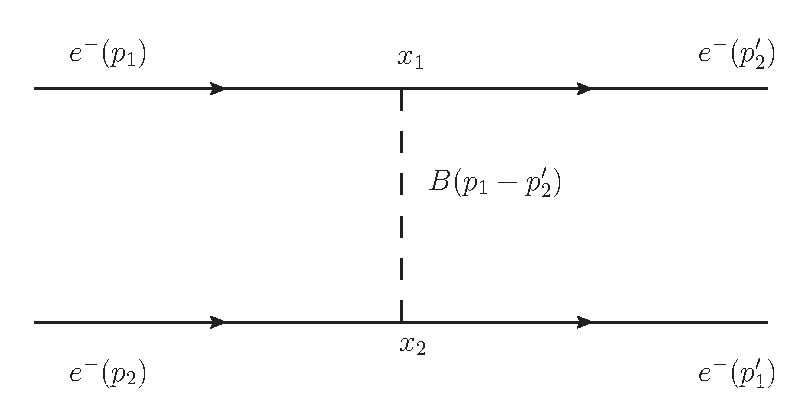
\includegraphics[scale=0.62]{scattering} %noinstiki
 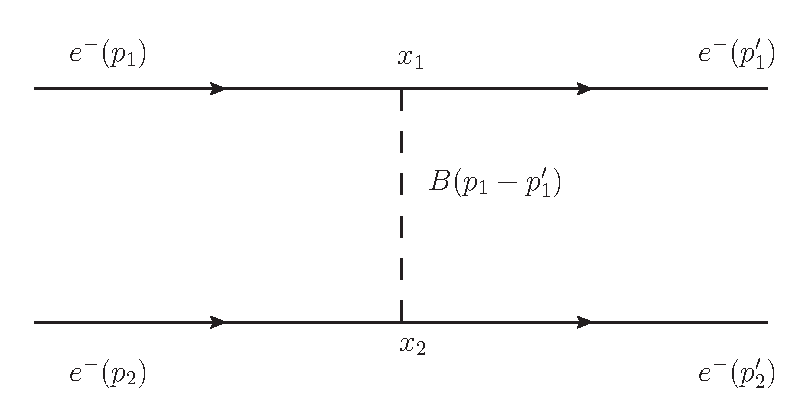
\includegraphics[scale=0.62]{scattering2} %noinstiki
  \caption{fermion scattering (Not Weyl fermion notation yet)} %noinstiki
  \label{fig:sct} %noinstiki
\end{figure} %noinstiki

%Calculates now the cross section

To calculate the corresponding cross section, we must start by calculating
\begin{align}
  \mathcal{M}\mathcal{M}^{\dagger}=&
y^4\left[
y^{\alpha}(\mathbf{p}_1')y^{\beta}(\mathbf{p}_2')\Delta_F(p_1-p_1')x_{\alpha}(\mathbf{p}_1)x_{\beta}(\mathbf{p}_2)   
  - y^{\alpha}(\mathbf{p}_2')y^{\beta}(\mathbf{p}_1')\Delta_F(p_1-p_2')x_{\alpha}(\mathbf{p}_1)x_{\beta}(\mathbf{p}_2)
\right] \nonumber\\
&\times\left[
x_{\dot{\beta}}^{\dagger}(\mathbf{p}_2)x_{\dot{\alpha}}^{\dagger}(\mathbf{p}_1)\Delta_F(p_1-p_1')y^{\dagger\dot{\beta}} (\mathbf{p}_2') y^{\dagger\dot{\alpha}}(\mathbf{p}_1')
  - x_{\dot{\beta}}^{\dagger}(\mathbf{p}_2)x_{\dot{\alpha}}^{\dagger}(\mathbf{p}_1)\Delta_F(p_1-p_2')y^{\dagger\dot{\beta}}(\mathbf{p}_1')y^{\dagger\dot{\alpha}}(\mathbf{p}_2')
\right]
\end{align}
\begin{align}
  =&y^4 \Delta_F^2(p_1-p_1')\left[y^{\alpha}(\mathbf{p}_1')y^{\beta}(\mathbf{p}_2')x_{\alpha}(\mathbf{p}_1)x_{\beta}(\mathbf{p}_2) 
x_{\dot{\beta}}^{\dagger}(\mathbf{p}_2)x_{\dot{\alpha}}^{\dagger}(\mathbf{p}_1)y^{\dagger\dot{\beta}} (\mathbf{p}_2') y^{\dagger\dot{\alpha}}(\mathbf{p}_1')  \right] \nonumber\\
&+y^4 \Delta_F^2(p_1-p_2') \left[
  \right] \nonumber\\
&-y^4\Delta_F(p_1-p_1')\Delta_F(p_1-p_2') \left[ \right. \nonumber\\
    &\left.  \right].
\end{align}

For the first term in the expansion and taking into account summming over spins, we have
\begin{align}
 \left| \mathcal{M}_1 \right| = &y^4 \Delta_F^2(p_1-p_2')\, \sum_{\text{spins}}y^{\alpha}(\mathbf{p}_1')y^{\beta}(\mathbf{p}_2')x_{\alpha}(\mathbf{p}_1)x_{\beta}(\mathbf{p}_2) 
x_{\dot{\beta}}^{\dagger}(\mathbf{p}_2)x_{\dot{\alpha}}^{\dagger}(\mathbf{p}_1)y^{\dagger\dot{\beta}} (\mathbf{p}_2') y^{\dagger\dot{\alpha}}(\mathbf{p}_1') 
\end{align}
Using \eqref{eq:xxd}
\begin{align}
  \left| \mathcal{M}_1 \right|^2 = &y^4 \Delta_F^2(p_1-p_2')\,p_2\cdot \sigma_{\beta\dot{\beta}} x_{\dot{\alpha}}^{\dagger}  \sum_{\text{spins}}y^{\alpha}(\mathbf{p}_1')y^{\beta}(\mathbf{p}_2') x_{\alpha}(\mathbf{p}_1)(\mathbf{p}_1)y^{\dagger\dot{\beta}} (\mathbf{p}_2') y^{\dagger\dot{\alpha}}(\mathbf{p}_1') \nonumber\\
= &y^4 \Delta_F^2(p_1-p_2')\, p_2\cdot \sigma_{\beta\dot{\beta}}\, p_1\cdot \sigma_{\alpha\dot{\alpha}}   \sum_{\text{spins}}y^{\alpha}(\mathbf{p}_1')y^{\beta}(\mathbf{p}_2') y^{\dagger\dot{\beta}} (\mathbf{p}_2') y^{\dagger\dot{\alpha}}(\mathbf{p}_1') \nonumber\\
 = &y^4 \Delta_F^2(p_1-p_2')\, p_2\cdot \sigma_{\beta\dot{\beta}}\,p_2'\cdot \overline{\sigma}^{\dot{\beta}\beta}\, p_1\cdot \sigma_{\alpha\dot{\alpha}}\,   \sum_{\text{spins}}y^{\alpha}(\mathbf{p}_1') y^{\dagger\dot{\alpha}}(\mathbf{p}_1') \nonumber\\
= &y^4 \Delta_F^2(p_1-p_2')\, p_2\cdot \sigma_{\beta\dot{\beta}}\,p_2'\cdot \overline{\sigma}^{\dot{\beta}\beta}\, p_1\cdot \sigma_{\alpha\dot{\alpha}}   \,p_1'\cdot \overline{\sigma}^{\dot{\alpha}\alpha}    \nonumber\\
= &y^4 \Delta_F^2(p_1-p_2')\,\operatorname{Tr} \left[ p_1\cdot \sigma   \,p_1'\cdot \overline{\sigma} \right]  \operatorname{Tr}\left[p_2\cdot\sigma\,p_2'\cdot \overline{\sigma}  \right],
\end{align}
By using \eqref{eq:trss}
\begin{align}
  \left| \mathcal{M}_1 \right|^2 = & y^4  \Delta_F^2(p_1-p_2')\,p_1^{\mu}{p_1'}^{\nu}\operatorname{Tr} \left[  \sigma^{\mu}  \overline{\sigma}^{\nu} \right] p_2^{\mu}{p_2'}^{\nu} \operatorname{Tr}\left[\sigma^{\mu} \overline{\sigma}^{\nu} \right]\nonumber\\
= & 2y^4  \frac{\left( p_1\cdot p_1' \right) \left( p_2\cdot{p_2'} \right).}{\left[ \left(p_1-p_2'\right)^2-m^2_h \right]^2}\,
\end{align}
where we also have used
\begin{align}
  \Delta_F(q)=\frac{1}{q^2-m^2}
\end{align}
We can generalize the defintion of $s$ in eq.\eqref{eq:smv} to the full
Mandelstam variables \url{http://bolvan.ph.utexas.edu/~vadim/Classes/2011f/STU.pdf},
\begin{align}
  s=&\left( p_1+p_2 \right)^2=\left( p_1'+p_2' \right)^2 \nonumber\\
  t=&\left( p_1-p_1' \right)^2=\left( p_2-p_2' \right)^2 \nonumber\\
  u=&\left( p_1-p_2' \right)^2=\left( p_1'-p_2 \right)^2 \,.
\end{align}
The explicit form for $s$ is
\begin{align}
  s=&\left( p_1+p_2 \right)^2 \nonumber\\
 =& p_1^2+p_2^2+2 p_1\cdot p_2 \nonumber\\
=& m_1^2+m_2^2+2 p_1\cdot p_2\,,
\end{align}
from which the product $p_1\cdot p_2$ can be obtained.  By following similar steps for $t$ and $u$, we have
\begin{align}
  2 p_1\cdot p_2=&s- m_1^2-m_2^2 \nonumber\\
  2 p_1'\cdot p_2'=&s- {m_1'}^2-{m_2'}^2 \nonumber\\
  2 p_1\cdot p_1'=&m_1^2+{m_1'}^2 -t \nonumber\\
  2 p_2\cdot p_2'=&m_2^2+{m_2'}^2 -t \nonumber\\
  2 p_1\cdot p_2'=&m_1^2+{m_2'}^2 -u \nonumber\\
  2 p_2\cdot p_1'=&m_2^2+{m_1'}^2 -u \,.
\end{align}
Moreover,
\begin{align}
  s+t+u=m_1^2+m_2^2+{m_1'}^2+{m_2'}^2\,.
\end{align}

Then, we can get the product of crossed momentum in terms of $t$
\begin{align}
  \left| \mathcal{M}_1 \right|^2 = & \frac{y^4}{2}  \frac{ \left(m_1^2+{m_1'}^2-t  \right)\left( m_2^2+{m_2'}^2-t \right)}{\left[ u-m^2_h \right]^2}
\end{align}
By using the general formula for the $2\to 2$ cross section in eq.~\eqref{eq:}
\begin{align}
  \frac{d\sigma}{d\Omega}=&\frac{1}{64\pi^2s}
\frac{\lambda^{1/2}(s,{m_2'}^2,{m_1'}^2)}{\lambda^{1/2}(s,m_2^2,m_1^2)}
\overline{|\mathcal{M}|^2} \nonumber\\
=&\frac{y^4}{128\pi^2s}
\frac{\lambda^{1/2}(s,{m_2'}^2,{m_1'}^2)}{\lambda^{1/2}(s,m_2^2,m_1^2)}
 \frac{ \left(m_1^2+{m_1'}^2-t  \right)\left( m_2^2+{m_2'}^2-t \right)}{\left[ u-m^2_h \right]^2}
\end{align}

We have that for Higgs couplings
\begin{align}
  m_1=&m_1'\,,&m_2=&m_2'\,,
\end{align}
therefore
\begin{align}
    \frac{d\sigma}{d\Omega}
=&\frac{y^4}{128\pi^2s}
  \frac{ \left(2m_1^2-t  \right)\left( 2m_2^2-t \right)}{\left[m^2_h -u\right]^2}
\end{align}
In the low energy limit we have
\begin{align}
  p_i=\left(m_i,\mathbf{p}_i  \right)
\end{align}
Therefore
\begin{align}
  \frac{d\sigma}{d\Omega}=&\frac{y^4}{128 \pi^2 \left[ \left(m_1+m_2 \right)^2+\left( \mathbf{p}_1+\mathbf{p_2} \right)^2 \right]}\frac{\left( 2m_1^2 \right)\left( 2m_2^2 \right)}{
\left[ m_h^2-\left(m_1-m_2  \right)^2 \right]^2} \nonumber\\
  \frac{d\sigma}{d\Omega}=&\frac{y^4}{128 \pi^2 }\frac{4m_1^2m_2^2}{\left(m_1+m_2 \right)^2}\frac{1}{
 m_h^4-2m_h^{2}\left(m_1-m_2  \right)^2+\left(m_1-m_2  \right)^4 } \nonumber\\
\end{align}

When the two particles are distinguishable: For example if the spin of $q_L$ is $s_2$ and $s'$ and the spin of $e_L$ is $s_{1}$ and $s$, then %recalculate
\begin{align}
  \xi^\alpha_{e+}(x_1)\xi^\beta_{q+}(x_2)|q_L(\mathbf{p}_2)e_L(\mathbf{p}_1)\rangle=&
\int\frac{d^3k}{(2\pi)^3\sqrt{2E_k V}}\int\frac{d^3k'}{(2\pi)^3\sqrt{2E_{k'}V}}
x^\alpha_e(s,\mathbf{k})x^\beta_q(s',\mathbf{k}')\operatorname{e}^{-i k\cdot x_1}\operatorname{e}^{-i k'\cdot x_2}\nonumber\\
&\times a_s(\mathbf{k})a_{s'}(\mathbf{k}')a_{s_1}^\dagger(\mathbf{p}_1)a_{s_2}^\dagger(\mathbf{p}_2)|0\rangle \nonumber\\
=&
\int\frac{d^3k'}{(2\pi)^3\sqrt{2E_k V}}\int\frac{d^3k}{(2\pi)^3\sqrt{2E_{k'}V}}
x^\alpha_e(s,\mathbf{k})x^\beta_q(s',\mathbf{k}')\operatorname{e}^{-i k\cdot x_1}\operatorname{e}^{-i k'\cdot x_2}\nonumber\\
&\times \left[ a_s(\mathbf{k})a_{s'}(\mathbf{k}')a_{s_1}^\dagger(\mathbf{p}_1)a_{s_2}^\dagger(\mathbf{p}_2) - a_{s_1}^\dagger(\mathbf{p}_1)a_{s_2}^\dagger(\mathbf{p}_2) a_s(\mathbf{k})a_{s'}(\mathbf{k}') \right]|0\rangle \nonumber\\
=&
\int\frac{d^3k}{(2\pi)^3\sqrt{2E_k V}}\int\frac{d^3k'}{(2\pi)^3\sqrt{2E_{k'}V}}
x^\alpha_e(s,\mathbf{k})x^\beta_q(s',\mathbf{k}')\operatorname{e}^{-i k\cdot x_1}\operatorname{e}^{-i k'\cdot x_2}\nonumber\\
&\times \left[ a_s(\mathbf{k})a_{s'}(\mathbf{k}'),a_{s_1}^\dagger(\mathbf{p}_1)a_{s_2}^\dagger(\mathbf{p}_2)\right]|0\rangle.
\end{align}
By using the identity
\begin{align}
  [AB,CD]=A[B,C]D - [A,C]BD
+CA[B, D] - C[A, D]B\,,
\end{align}
\begin{align}
   \left[ a_s(\mathbf{k})a_{s'}(\mathbf{k}'),a_{s_1}^\dagger(\mathbf{p}_1)a_{s_2}^\dagger(\mathbf{p}_2)\right]=&
 a_s(\mathbf{k})\cancel{\left[ a_{s'}(\mathbf{k}'),a_{s_1}^\dagger(\mathbf{p}_1)\right]}a_{s_2}^\dagger(\mathbf{p}_2)
-
 \left[ a_s(\mathbf{k}),a_{s_1}^\dagger(\mathbf{p}_1)\right]a_{s'}(\mathbf{k}')a_{s_2}^\dagger(\mathbf{p}_2) \nonumber\\
& 
+a_{s_1}^\dagger(\mathbf{p}_1)a_s(\mathbf{k})\left[ a_{s'}(\mathbf{k}'),a_{s_2}^\dagger(\mathbf{p}_2)\right]
-
a_{s_1}^\dagger(\mathbf{p}_1) \cancel{\left[ a_s(\mathbf{k}),a_{s_2}^\dagger(\mathbf{p}_2)\right]}a_{s'}(\mathbf{k}') \nonumber\\
=&
-
 \left[ a_s(\mathbf{k}),a_{s_1}^\dagger(\mathbf{p}_1)\right]a_{s'}(\mathbf{k}')a_{s_2}^\dagger(\mathbf{p}_2)  
+\left[ a_{s'}(\mathbf{k}'),a_{s_2}^\dagger(\mathbf{p}_2)\right]a_{s_1}^\dagger(\mathbf{p}_1)a_s(\mathbf{k})
\end{align}
Therefore,
\begin{align}
&\left[ a_s(\mathbf{k})a_{s'}(\mathbf{k}'),a_{s_1}^\dagger(\mathbf{p}_1)a_{s_2}^\dagger(\mathbf{p}_2)\right] |0\rangle \nonumber\\
&\qquad=
-
 \left[ a_s(\mathbf{k}),a_{s_1}^\dagger(\mathbf{p}_1)\right]a_{s'}(\mathbf{k}')a_{s_2}^\dagger(\mathbf{p}_2) |0\rangle \nonumber\\
&\qquad=-
  \left[ a_s(\mathbf{k}),a_{s_1}^\dagger(\mathbf{p}_1)\right] \left[ a_{s'}(\mathbf{k}'),a_{s_2}^\dagger(\mathbf{p}_2)  \right] |0\rangle \nonumber\\
&\qquad= -(2\pi)^6  
    \delta^{(3)}(\mathbf{k}-\mathbf{p}_1)\delta^{(3)}(\mathbf{k}'-\mathbf{p}_2)|0\rangle
\end{align}
The final result following the same steps is
\begin{align}
\label{eq:hdee}
     S_{fi}
    =\frac{(2\pi)^4(iy)^2\delta^{(4)}\left(p_1+p_2-p_1'-p_2'\right) }{\sqrt{2 E_1'V}\sqrt{2 E_2'V}\sqrt{2 E_1V}\sqrt{2 E_2V}}
  &\left[ y^{\alpha}_e(\mathbf{p}_1')y^{\beta}_q(\mathbf{p}_2')i\Delta_F(p_1-p_1')x_{e \alpha}(\mathbf{p}_1)x_{q \beta}(\mathbf{p}_2)\right].
\end{align}



Others possibilities for two intial particle states includes
\begin{align}
  |e_R(\mathbf{p}_2)e_L(\mathbf{p}_1)\rangle=&\frac{1}{\sqrt{V^2}}a_{s_1}^\dagger(\mathbf{p}_1)a_{s_2}^\dagger(\mathbf{p}_2)|0\rangle
\end{align}

Following similar steps, we find for
\begin{align}
\eta^{\dagger\dot{\alpha}}_+(x_1)&\xi^{\alpha}_+(x_2)|e_R(\mathbf{p}_2)e_L(\mathbf{p}_1)\rangle
 \nonumber\\
\label{eq:berer}
&=\frac{1 }{\sqrt{2 E_1V}\sqrt{2 E_2V}} \left[ y^{\dagger\dot{\alpha}}(\mathbf{p}_2)x^{\alpha}(\mathbf{p}_1)
\operatorname{e}^{-i p_2\cdot x_1}\operatorname{e}^{-i p_1\cdot x_2}
-y^{\dagger\dot{\alpha}}(\mathbf{p}_1)x^{\alpha}(\mathbf{p}_2)
\operatorname{e}^{-i p_1\cdot x_1}\operatorname{e}^{-i p_2\cdot x_2}   \right] \left|0\right\rangle \\
\langle e_R(\mathbf{p}_2)&e_L(\mathbf{p}_1)| \xi^{\dagger\dot{\alpha}}_-(x_1)\eta^{\alpha}_-(x_2)
 \nonumber\\
\label{eq:berer}
&=\left\langle 0\right|\frac{1 }{\sqrt{2 E_1V}\sqrt{2 E_2V}} \left[ x^{\dagger\dot{\alpha}}(\mathbf{p}_2)y^{\beta}(\mathbf{p}_1)
\operatorname{e}^{i p_2\cdot x_1}\operatorname{e}^{i p_1\cdot x_2}
- x^{\dagger\dot{\alpha}}(\mathbf{p}_1)y^{\alpha}(\mathbf{p}_2)
\operatorname{e}^{i p_1\cdot x_1}\operatorname{e}^{i p_2\cdot x_2}   \right].
\end{align}


Consider now



\begin{align}
  |\left( e_L \right)^{\dagger}(\mathbf{p}_2)e_L(\mathbf{p}_1)\rangle=&\frac{1}{\sqrt{V^2}}a_{s_1}^\dagger(\mathbf{p}_1)b_{s_2}^\dagger(\mathbf{p}_2)|0\rangle
\end{align}


Therefore, the spin of $\left(e_L\right)^{\dagger}$ is $s_2$ and $s'$ and the spin of $e_L$ is $s_{1}$ and $s$, then %recalculate
\begin{align}
  \xi^\alpha_{+}(x_1)\xi^{\dagger\dot{\alpha}}_{+}x(x_2)|\left(e_L\right)^{\dagger}(\mathbf{p}_2)e_L(\mathbf{p}_1)\rangle=&
\int\frac{d^3k}{(2\pi)^3\sqrt{2E_k V}}\int\frac{d^3k'}{(2\pi)^3\sqrt{2E_{k'}V}}
x^\alpha(s,\mathbf{k})y^{\dagger\dot{\alpha}}(s',\mathbf{k}')\operatorname{e}^{-i k\cdot x_1}\operatorname{e}^{-i k'\cdot x_2}\nonumber\\
&\times a_s(\mathbf{k})a_{s'}(\mathbf{k}')b_{s_1}^\dagger(\mathbf{p}_1)b_{s_2}^\dagger(\mathbf{p}_2)|0\rangle \nonumber\\
=&
\int\frac{d^3k'}{(2\pi)^3\sqrt{2E_k V}}\int\frac{d^3k}{(2\pi)^3\sqrt{2E_{k'}V}}
x^\alpha(s,\mathbf{k})y^{\dagger\dot{\alpha}}(s',\mathbf{k}')\operatorname{e}^{-i k\cdot x_1}\operatorname{e}^{-i k'\cdot x_2}\nonumber\\
&\times \left[ a_s(\mathbf{k})b_{s'}(\mathbf{k}')a_{s_1}^\dagger(\mathbf{p}_1)b_{s_2}^\dagger(\mathbf{p}_2) - a_{s_1}^\dagger(\mathbf{p}_1)b_{s_2}^\dagger(\mathbf{p}_2) b_s(\mathbf{k})a_{s'}(\mathbf{k}') \right]|0\rangle \nonumber\\
=&
\int\frac{d^3k}{(2\pi)^3\sqrt{2E_k V}}\int\frac{d^3k'}{(2\pi)^3\sqrt{2E_{k'}V}}
x^\alpha(s,\mathbf{k})y^{\dagger\dot{\alpha}}(s',\mathbf{k}')\operatorname{e}^{-i k\cdot x_1}\operatorname{e}^{-i k'\cdot x_2}\nonumber\\
&\times \left[ a_s(\mathbf{k})b_{s'}(\mathbf{k}'),a_{s_1}^\dagger(\mathbf{p}_1)b_{s_2}^\dagger(\mathbf{p}_2)\right]|0\rangle.
\end{align}
By using the identity
\begin{align}
  [AB,CD]=A[B,C]D - [A,C]BD
+CA[B, D] - C[A, D]B\,,
\end{align}
\begin{align}
   \left[ a_s(\mathbf{k})b_{s'}(\mathbf{k}'),a_{s_1}^\dagger(\mathbf{p}_1)b_{s_2}^\dagger(\mathbf{p}_2)\right]=&
 a_s(\mathbf{k})\cancel{\left[ b_{s'}(\mathbf{k}'),a_{s_1}^\dagger(\mathbf{p}_1)\right]}b_{s_2}^\dagger(\mathbf{p}_2)
-
 \left[ a_s(\mathbf{k}),a_{s_1}^\dagger(\mathbf{p}_1)\right]b_{s'}(\mathbf{k}')b_{s_2}^\dagger(\mathbf{p}_2) \nonumber\\
& 
+a_{s_1}^\dagger(\mathbf{p}_1)a_s(\mathbf{k})\left[ b_{s'}(\mathbf{k}'),b_{s_2}^\dagger(\mathbf{p}_2)\right]
-
a_{s_1}^\dagger(\mathbf{p}_1) \cancel{\left[ a_s(\mathbf{k}),b_{s_2}^\dagger(\mathbf{p}_2)\right]}b_{s'}(\mathbf{k}') \nonumber\\
=&
-
 \left[ a_s(\mathbf{k}),a_{s_1}^\dagger(\mathbf{p}_1)\right]b_{s'}(\mathbf{k}')b_{s_2}^\dagger(\mathbf{p}_2)  
+\left[ b_{s'}(\mathbf{k}'),b_{s_2}^\dagger(\mathbf{p}_2)\right]a_{s_1}^\dagger(\mathbf{p}_1)a_s(\mathbf{k})
\end{align}
Therefore,
\begin{align}
&\left[ a_s(\mathbf{k})b_{s'}(\mathbf{k}'),a_{s_1}^\dagger(\mathbf{p}_1)b_{s_2}^\dagger(\mathbf{p}_2)\right] |0\rangle \nonumber\\
&\qquad=
-
 \left[ a_s(\mathbf{k}),a_{s_1}^\dagger(\mathbf{p}_1)\right]b_{s'}(\mathbf{k}')b_{s_2}^\dagger(\mathbf{p}_2) |0\rangle \nonumber\\
&\qquad=-
  \left[ a_s(\mathbf{k}),a_{s_1}^\dagger(\mathbf{p}_1)\right] \left[ b_{s'}(\mathbf{k}'),b_{s_2}^\dagger(\mathbf{p}_2)  \right] |0\rangle \nonumber\\
&\qquad= -(2\pi)^6  
    \delta^{(3)}(\mathbf{k}-\mathbf{p}_1)\delta^{(3)}(\mathbf{k}'-\mathbf{p}_2)|0\rangle
\end{align}
Therefore
\begin{align}
\label{eq:bkeldel}
    \xi^\alpha_{+}(x_1)\xi^{\dagger\dot{\alpha}}_{+}(x_2)|\left(e_L\right)^{\dagger}(\mathbf{p}_2)e_L(\mathbf{p}_1)\rangle=&
-\frac{1}{\sqrt{2E_1 V}\sqrt{2E_2 V}}\,x^\alpha(s,\mathbf{p}_1)y^{\dagger\dot{\alpha}}(s',\mathbf{p}_2)\operatorname{e}^{-i p_1\cdot x_1}\operatorname{e}^{-i p_2\cdot x_2} \nonumber\\
   \left\langle\left(e_L\right)^{\dagger}(\mathbf{p}_2) e_L(\mathbf{p}_1) \right|\xi^{\alpha}_-(x_2)\xi^{\dagger\dot{\alpha}}_-\left( x_1 \right)=&
-\frac{1}{\sqrt{2E_1 V}\sqrt{2E_2 V}}\,y^{\alpha}(s',\mathbf{p}_2) x^{\dagger\dot{\alpha}}(s,\mathbf{p}_1)\operatorname{e}^{i p_1\cdot x_1}\operatorname{e}^{i p_2\cdot x_2}
\end{align}

\subsection{Vector interactions}



\subsubsection{Bahba scattering}

We consider the $t$-channel interaction
\begin{align}
  e_L+\left( e_L \right)^{\dagger} \to   e_L+\left( e_L \right)^{\dagger}
\end{align}
mediated by $A^{\mu}$, with couplings
\begin{align}
\label{eq:xietaz}
\mathcal{L}=e \xi^{\dagger}_{\dot{\alpha}}\left( \overline{\sigma}^{\mu} \right)^{\dot{\alpha}\alpha}\xi_{\alpha} A_{\mu}
+e \eta^{\alpha} \sigma^{\mu}_{\alpha\dot{\alpha}} \eta^{\dagger\dot{\alpha}} A_{\mu}
\end{align}

This is an explicit case for distinguishable particles


The specific calculation by the scattering mediated by the $A^{\mu}$ is 
\begin{align}
  S_{fi}=&\frac{\left( -ie \right)^{2}}{2!}\sum_{\text{spins}}\int\int \operatorname{d}^4x_1 \operatorname{d}^4x_2
\bcontraction{\,}{A_{\mu}}{(x_1)}{A_{\nu}}\,A_{\mu}(x_1)A_{\nu}(x_2) \nonumber\\
&\left\langle \left(e_L\right)^{\dagger} \left(\mathbf{p}'_2\right),e_L\left(\mathbf{p}'_1\right) \right|
  : \xi^{\dagger}_{\dot{\alpha}}(x_1)\left( \overline{\sigma}^{\mu} \right)^{\dot{\alpha}\alpha}\xi_{\alpha}(x_1)\xi^{\dagger}_{\dot{\beta}}(x_2)\left( \overline{\sigma}^{\nu} \right)^{\dot{\beta}\beta}\xi_{\beta}(x_2):
 \left| \left(e_L\right)^{\dagger}\left(\mathbf{p}_2\right) ,e_L \left(\mathbf{p}_1\right)  \right\rangle \nonumber\\
\end{align}
\begin{align}
  =&\frac{\left( -ie \right)^{2}}{2!}\sum_{\text{spins}}\int\int \operatorname{d}^4x_1 \operatorname{d}^4x_2
D_{\mu\nu} \left( x_1-x_2 \right)\nonumber\\
&\left\langle \left(e_L\right)^{\dagger} \left(\mathbf{p}'_2\right),e_L\left(\mathbf{p}'_1\right)\right|
   \xi_{\beta -}(x_2)\xi^{\dagger}_{\dot{\alpha} -}(x_1)\left( \overline{\sigma}^{\mu} \right)^{\dot{\alpha}\alpha}\left( \overline{\sigma}^{\nu} \right)^{\dot{\beta}\beta}\xi_{\alpha +}(x_1)\xi^{\dagger}_{\dot{\beta}+}(x_2)
 \left| \left(e_L\right)^{\dagger}\left(\mathbf{p}_2\right), e_L \left(\mathbf{p}_1\right)\right\rangle. 
\end{align}


\begin{align}
  S_{fi}
=&\frac{\left( -ie \right)^{2}}{2!}\frac{1}{\sqrt{2E_1' V}\sqrt{2E_2' V}\sqrt{2E_1 V}\sqrt{2E_2 V}}
\sum_{\text{spins}}\int\int \operatorname{d}^4x_1 \operatorname{d}^4x_2
D_{\mu\nu} \left( x_1-x_2 \right)\nonumber\\
&y_{\beta}\left(s'_2,\mathbf{p}_2'\right)x^{\dagger}_{\dot{\alpha}}\left( s'_1,\mathbf{p}_1' \right)
\left( \overline{\sigma}^{\mu} \right)^{\dot{\alpha}\alpha}\left( \overline{\sigma}^{\nu} \right)^{\dot{\beta}\beta}
x_{\alpha}\left(s_1,\mathbf{p}_1\right)y^{\dagger}_{\dot{\beta}}\left( s_2,\mathbf{p}_2 \right)
\operatorname{e}^{i p_1'\cdot x_1}\operatorname{e}^{i p_2'\cdot x_2}
\operatorname{e}^{-i p_1\cdot x_1}\operatorname{e}^{-i p_2\cdot x_2}\,.
\end{align}


By using \eqref{eq:bkeldel}, we have an expression similar to \eqref{eq:hdee}, and following the same steps
\begin{align}
      S_{fi}
    =&\frac{(2\pi)^4(ie)^2\delta^{(4)}\left(p_1+p_2-p_1'-p_2'\right) }{\sqrt{2 E_1'V}\sqrt{2 E_2'V}\sqrt{2 E_1V}\sqrt{2 E_2V}}
 \left[ x^{\dagger}_{\dot{\alpha}}(\mathbf{p}_1')\left( \overline{\sigma}^{\mu} \right)^{\dot{\alpha}\alpha}x_{\alpha}(\mathbf{p}_1)  i D_{\mu\nu}y^{\dagger}_{\dot{\beta}}(\mathbf{p}_2) \left( \overline{\sigma}^{\nu} \right)^{\dot{\beta}\beta}y_{\beta}(\mathbf{p}_2')\right] \nonumber\\
    =&\frac{(2\pi)^4(ie)^2\delta^{(4)}\left(p_1+p_2-p_1'-p_2'\right) }{\sqrt{2 E_1'V}\sqrt{2 E_2'V}\sqrt{2 E_1V}\sqrt{2 E_2V}}
 \left[ x^{\dagger}(\mathbf{p}_1') \overline{\sigma}^{\mu}x(\mathbf{p}_1)  i D_{\mu\nu}y^{\dagger}(\mathbf{p}_2) \overline{\sigma}^{\nu} y(\mathbf{p}_2')\right] \nonumber\\
    =&\frac{(2\pi)^4(ie)^2\delta^{(4)}\left(p_1+p_2-p_1'-p_2'\right) }{\sqrt{2 E_1'V}\sqrt{2 E_2'V}\sqrt{2 E_1V}\sqrt{2 E_2V}}
 \left[ x(\mathbf{p}_1) {\sigma}^{\mu}x^{\dagger}(\mathbf{p}_1')  i D_{\mu\nu}y^{\dagger}(\mathbf{p}_2) \overline{\sigma}^{\nu} y(\mathbf{p}_2')\right],
\end{align}
where we use the identity for commuting spinors.

In this way %eq. 6.3.6  pag. 51
\begin{align}
  i\mathcal{M}=&e^2\left[ x(\mathbf{p}_1) {\sigma}^{\mu}x^{\dagger}(\mathbf{p}_1')  i D_{\mu\nu}y^{\dagger}(\mathbf{p}_2) \overline{\sigma}^{\nu} y(\mathbf{p}_2')\right]
\end{align}
If in addtion we include the other three possibilites in the $t$-channel, by defining
\begin{align}
 \overline{e}=&\left( e_R \right)^{\dagger}\,, & \overline{e}^{\dagger}=&e_R\,,
\end{align}
then, we have the full contributions
\begin{align}
 e_L+\left( e_L \right)^{\dagger} \to &  e_L+\left( e_L \right)^{\dagger}\,, & e_R+\left( e_R \right)^{\dagger} \to &  e_R+\left( e_R \right)^{\dagger}\,, \nonumber\\
  e_L+\left( e_R \right)^{\dagger}\to &  e_L+\left( e_R \right)^{\dagger}\,, &  e_R+\left( e_L \right)^{\dagger}\to & e_R+\left( e_L \right)^{\dagger} \,,
\end{align}
which give the full $t$-channel amplitude \cite{Dreiner:2008tw} eq.~(6.3.6), pag. 51:
\begin{align}
   i\mathcal{M}=&e^2\left[ x(\mathbf{p}_1) {\sigma}^{\mu}x^{\dagger}(\mathbf{p}_1') + y^{\dagger}(\mathbf{p}_1) \overline{\sigma}^{\nu} y(\mathbf{p}_1')\right]i D_{\mu\nu}\left[ x(\mathbf{p}_2) {\sigma}^{\mu}x^{\dagger}(\mathbf{p}_2') + y^{\dagger}(\mathbf{p}_2) \overline{\sigma}^{\nu} y(\mathbf{p}_2')  \right]\,.
\end{align}


\subsubsection{Lepton quark scattering}

mediated by $Z^{\mu}$, with couplings
\begin{align}
\label{eq:xietaz}
\mathcal{L}=a_L \xi^{\dagger}_{\dot{\alpha}}\left( \overline{\sigma}^{\mu} \right)^{\dot{\alpha}\alpha}\xi_{\alpha} Z_{\mu}
+b_L \eta^{\alpha} \sigma^{\mu}_{\alpha\dot{\alpha}} \eta^{\dagger\dot{\alpha}} Z_{\mu}
\end{align}

We now consider the interaction
\begin{align}
  e_L+q_L \to e_L+q_L
\end{align}
We have then the two particle state but with distinguishable particles 

The specific calculation by the scattering mediated by the $Z^{\mu}$ is 
\begin{align}
  S_{fi}=&\frac{\left( -ia_L \right)^{2}}{2!}\sum_{\text{spins}}\int\int \operatorname{d}^4x_1 \operatorname{d}^4x_2
\bcontraction{\,}{Z_{\mu}}{(x_1)}{Z_{\nu}}\,Z_{\mu}(x_1)Z_{\nu}(x_2) \nonumber\\
&\left\langle q_L \left(\mathbf{p}'_2\right),e_L\left(\mathbf{p}'_1\right) \right|
  : \xi^{\dagger}_{\dot{\alpha}}(x_1)\left( \overline{\sigma}^{\mu} \right)^{\dot{\alpha}\alpha}\xi_{\alpha}(x_1)\xi^{\dagger}_{\dot{\beta}}(x_2)\left( \overline{\sigma}^{\mu} \right)^{\dot{\beta}\beta}\xi_{\beta}(x_2):
 \left| q_L\left(\mathbf{p}_2\right) ,e_L \left(\mathbf{p}_1\right)  \right\rangle \nonumber\\
=&\frac{\left( -ia_L \right)^{2}}{2!}\sum_{\text{spins}}\int\int \operatorname{d}^4x_1 \operatorname{d}^4x_2
D_{\mu\nu} \left( x_1-x_2 \right)\nonumber\\
&\left\langle q_L \left(\mathbf{p}'_2\right),e_L\left(\mathbf{p}'_1\right)\right|
   \xi^{\dagger}_{\dot{\alpha} -}(x_1)\xi^{\dagger}_{\dot{\beta}-}(x_2)\left( \overline{\sigma}^{\mu} \right)^{\dot{\alpha}\alpha}\left( \overline{\sigma}^{\mu} \right)^{\dot{\beta}\beta}\xi_{\alpha +}(x_1)\xi_{\beta +}(x_2)
 \left| q_L\left(\mathbf{p}_2\right), e_L \left(\mathbf{p}_1\right)\right\rangle. 
\end{align}



By using~\eqref{eq:belel}, \eqref{eq:kelel}, we have an expression similar to \eqref{eq:hdee}
\begin{align}
      S_{fi}
    =&\frac{(2\pi)^4(ia_L)^2\delta^{(4)}\left(p_1+p_2-p_1'-p_2'\right) }{\sqrt{2 E_1'V}\sqrt{2 E_2'V}\sqrt{2 E_1V}\sqrt{2 E_2V}}
 \left[ x^{\dagger\dot{\alpha}}_e(\mathbf{p}_1')\left( \overline{\sigma}^{\mu} \right)^{\dot{\alpha}\alpha}x_{e \alpha}(\mathbf{p}_1)  i D_{\mu\nu}x^{\dagger\dot{\beta}}_q(\mathbf{p}_2') \left( \overline{\sigma}^{\nu} \right)^{\dot{\beta}\beta}x_{q \beta}(\mathbf{p}_2)\right] \nonumber\\
=&\frac{(2\pi)^4(ia_L)^2\delta^{(4)}\left(p_1+p_2-p_1'-p_2'\right) }{\sqrt{2 E_1'V}\sqrt{2 E_2'V}\sqrt{2 E_1V}\sqrt{2 E_2V}}
  \left[ x_e^{\dagger}(\mathbf{p}_1') \overline{\sigma}^{\mu}x_e(\mathbf{p}_1)  i D_{\mu\nu}x_q^{\dagger}(\mathbf{p}_2') \overline{\sigma}^{\nu} x_q(\mathbf{p}_2)\right].
\end{align}
In this way
\begin{align}
  \mathcal{M}=&(ia_L)^2 x_e^{\dagger}(\mathbf{p}_1') \overline{\sigma}^{\mu}x_e(\mathbf{p}_1)  i D_{\mu\nu}x_q^{\dagger}(\mathbf{p}_2') \overline{\sigma}^{\nu} x_q(\mathbf{p}_2)
\end{align}
\begin{align}
  \mathcal{M}\mathcal{M}^{\dagger}=&\sum_{\text{spins}}
a_L^4 x_e^{\dagger}(\mathbf{p}_1') \overline{\sigma}^{\mu}x_e(\mathbf{p}_1)   D_{\mu\nu}x_q^{\dagger}(\mathbf{p}_2') \overline{\sigma}^{\nu} x_q(\mathbf{p}_2) 
x_q^{\dagger}(\mathbf{p}_2) \overline{\sigma}^{\rho} x_q(\mathbf{p}_2') D_{\rho\sigma}
x_e^{\dagger}(\mathbf{p}_1) \overline{\sigma}^{\sigma}x_e(\mathbf{p}_1')
\end{align}
\begin{align}
  \mathcal{M}\mathcal{M}^{\dagger} =&\sum_{\text{spins}}
a_L^4 x_e^{\dagger}(\mathbf{p}_1') \overline{\sigma}^{\mu}x_e(\mathbf{p}_1)   D_{\mu\nu}x_q^{\dagger}(\mathbf{p}_2') \overline{\sigma}^{\nu} 
p_{2\delta}\sigma^{\delta} \overline{\sigma}^{\rho} x_q(\mathbf{p}_2') D_{\rho\sigma}
x_e^{\dagger}(\mathbf{p}_1) \overline{\sigma}^{\sigma}x_e(\mathbf{p}_1') \nonumber\\
=&\sum_{\text{spins}}a_L^4D_{\mu\nu} D_{\rho\sigma}  x_e^{\dagger\dot{\alpha}}(\mathbf{p}_1') \overline{\sigma}^{\mu}_{\dot{\alpha}\alpha}x_e^{\alpha}(\mathbf{p}_1)   x_q^{\dagger\dot{\beta}}(\mathbf{p}_2') \overline{\sigma}^{\nu}_{\dot{\beta}\beta} 
p_2 \cdot \sigma^{\beta\dot{\gamma}} \overline{\sigma}^{\rho}_{\dot{\gamma}\gamma} x_q^{\gamma}(\mathbf{p}_2')
x_e^{\dagger\dot{\delta}}(\mathbf{p}_1) \overline{\sigma}^{\sigma}_{\dot{\delta}\delta}x_e^{\delta}(\mathbf{p}_1') \nonumber\\
=&\sum_{\text{spins}}a_L^4D_{\mu\nu} D_{\rho\sigma} x_e^{\delta}(\mathbf{p}_1') x_e^{\dagger\dot{\alpha}}(\mathbf{p}_1') \overline{\sigma}^{\mu}_{\dot{\alpha}\alpha}x_e^{\alpha}(\mathbf{p}_1) x_e^{\dagger\dot{\delta}}(\mathbf{p}_1) \overline{\sigma}^{\sigma}_{\dot{\delta}\delta} x_q^{\gamma}(\mathbf{p}_2') x_q^{\dagger\dot{\beta}}(\mathbf{p}_2') \overline{\sigma}^{\nu}_{\dot{\beta}\beta} 
p_2\cdot \sigma^{\beta\dot{\gamma}} \overline{\sigma}^{\rho}_{\dot{\gamma}\gamma}  \nonumber\\
=&a_L^4D_{\mu\nu} D_{\rho\sigma} p_1'\cdot{\sigma}^{\delta\dot{\alpha}}   \overline{\sigma}^{\mu}_{\dot{\alpha}\alpha} p_1\cdot \sigma^{\alpha\dot{\delta}} \overline{\sigma}^{\sigma}_{\dot{\delta}\delta} p_2'\cdot {\sigma}^{\gamma\dot{\beta}}  \overline{\sigma}^{\nu}_{\dot{\beta}\beta} 
p_2\cdot \sigma^{\beta\dot{\gamma}} \overline{\sigma}^{\rho}_{\dot{\gamma}\gamma} 
\nonumber\\
=&a_L^4D_{\mu\nu} D_{\rho\sigma} \operatorname{Tr}\left[p_1'\cdot\sigma \overline{\sigma}^{\mu} p_1\cdot \sigma \overline{\sigma}^{\sigma}\right] 
               \operatorname{Tr}\left[p_2'\cdot \sigma \overline{\sigma}^{\nu} p_2\cdot \sigma \overline{\sigma}^{\rho}\right] 
\end{align}
\begin{align}
 \mathcal{M}\mathcal{M}^{\dagger}  =&a_L^4D_{\mu\nu} D_{\rho\sigma} {p_1}_{\lambda}{p_1'}_{\eta}{p_2}_{\tau}{p_2'}_{\theta}\operatorname{Tr}\left[\sigma^{\eta} \overline{\sigma}^{\mu}  \sigma^{\lambda} \overline{\sigma}^{\sigma}\right] 
               \operatorname{Tr}\left[\sigma^{\theta} \overline{\sigma}^{\nu} \sigma^{\tau} \overline{\sigma}^{\rho}\right] 
\end{align}
\begin{align}
  \operatorname{Tr}\left[\sigma^{\eta} \overline{\sigma}^{\mu}  \sigma^{\lambda} \overline{\sigma}^{\sigma}\right] &
               \operatorname{Tr}\left[\sigma^{\theta} \overline{\sigma}^{\nu} \sigma^{\tau} \overline{\sigma}^{\rho}\right] \nonumber\\
=& 4 \left(g^{\eta\mu}g^{\lambda\sigma}-g^{\eta\lambda}g^{\mu\sigma}+g^{\eta\sigma}g^{\mu\lambda} +i\epsilon^{\eta\mu\lambda\sigma} \right)
   \left(g^{\theta\nu}g^{\tau\rho}-g^{\theta\tau}g^{\nu\rho}+g^{\theta\rho}g^{\nu\tau} +i\epsilon^{\theta\nu\tau\rho} \right).
\end{align}
\begin{align}
\tfrac{1}{4} \operatorname{Tr}\left[\sigma^{\eta} \overline{\sigma}^{\mu}  \sigma^{\lambda} \overline{\sigma}^{\sigma}\right] 
\operatorname{Tr}\left[\sigma^{\theta} \overline{\sigma}^{\nu} \sigma^{\tau} \overline{\sigma}^{\rho}\right] 
  =&\phantom{-}g^{\eta\mu}g^{\lambda\sigma}g^{\theta\nu}g^{\tau\rho}-g^{\eta\mu}g^{\lambda\sigma}g^{\theta\tau}g^{\nu\rho}+g^{\eta\mu}g^{\lambda\sigma}g^{\theta\rho}g^{\nu\tau} \nonumber\\
  &-g^{\eta\lambda}g^{\mu\sigma}g^{\theta\nu}g^{\tau\rho}+g^{\eta\lambda}g^{\mu\sigma}g^{\theta\tau}g^{\nu\rho}-g^{\eta\lambda}g^{\mu\sigma}g^{\theta\rho}g^{\nu\tau} \nonumber\\
  &+g^{\eta\sigma}g^{\mu\lambda}g^{\theta\nu}g^{\tau\rho}-g^{\eta\sigma}g^{\mu\lambda}g^{\theta\tau}g^{\nu\rho}+g^{\eta\sigma}g^{\mu\lambda}g^{\theta\rho}g^{\nu\tau} 
%  =& 4 \left(g^{\eta\mu}g^{\lambda\sigma}-g^{\eta\lambda}g^{\mu\sigma}+g^{\eta\sigma}g^{\mu\lambda} +i\epsilon^{\eta\mu\lambda\sigma} \right)
%   \left(g^{\theta\nu}g^{\tau\rho}-g^{\theta\tau}g^{\nu\rho}+g^{\theta\rho}g^{\nu\tau} +i\epsilon^{\theta\nu\tau\rho} \right).
\end{align}
The $\epsilon$'s always appears along symmetric product and add 0.

Therefore, eliminating $\eta,\theta$, we have \begin{align}{p_1}_{\lambda}{p_1'}_{\eta}{p_2}_{\tau}{p_2'}_{\theta}\end{align}
% \begin{align} %Inconsistent!
%    \mathcal{M}\mathcal{M}^{\dagger} =&a_L^4 [
%  D_{\mu\nu} {p_1}^{\sigma}{p_1'}^{\mu}D_{\rho\sigma}{p_2}^{\rho}{p__2'}^{\nu}
% -{p_1}^{\sigma}{p_1'}^{\mu}{p_2}^{\theta}{p__2'}^{\nu}
% +{p_1}^{\sigma}{p_1'}^{\mu}{p_2}^{\nu}{p__2'}^{\rho}
% -{p_1}^{\lambda}{p_1'}^{a}{p_2}^{a}{p__2'}^{a}
% +{p_1}^{a}{p_1'}^{a}{p_2}^{a}{p__2'}^{a}
% ]
% \end{align}
For the interaction of a fermion pair with $W_\mu^\pm$, we know from
the standard model Lagrangian \cite{lsm}, that
\begin{align}
  \frac{g^2}{2\sqrt{2}}\overline{\psi}\gamma^\mu(1-\gamma_5)\psi
\end{align}
Therefore in this case
\begin{align}
  \Gamma=\gamma^\mu(1-\gamma_5)
\end{align}
For $p\ll M_W^2$ the analysis is similar to the previous one with
\begin{align}
   \bcontraction{\,}{W^\mu}{(x_1)}{W^\nu}
\,W^\mu(x_1)W^\nu(x_2)=&\langle0|T\{W^\mu(x_1)W^\nu(x_2)\}|0\rangle\nonumber\\
\approx&\int\frac{d^4q}{(2\pi)^4}\frac{g^{\mu\nu}}{M_W^2}e^{-i q\cdot(x_1-x_2)}
\end{align}

For the process 
\begin{align}
  e^-(p)+\nu_\mu(k)\to\mu^-(p')+\nu_e(k')
\end{align}
the global coupling for $p\ll M_W^2$ is
\begin{align}
  \frac{g^2}{8M_W^2}=&\frac{G_F}{\sqrt{2}}
\end{align}

After the replacement $G_F/\sqrt{2}\equiv h^2/m^2$, we have
\begin{align}
  \label{eq:101f}
  S^{(2)}_{fi}=i(2\pi)^4\delta^{4}\left(p_1+p_2-p'_1-p'_2\right)
  \frac{1}{\sqrt{2E_1 V}}\frac{1}{\sqrt{2E_2 V}}
  \frac{1}{\sqrt{2E_1' V}}\frac{1}{\sqrt{2E_2' V}}
  \mathcal{M}_{fi}
\end{align}
where
\begin{align}
  \mathcal{M}_{fi}=\frac{G_F}{\sqrt{2}}
\bar{u}_{\nu_e}(\mathbf{p}'_2)\Gamma u_e(\mathbf{p}_1)\bar{u}_\mu(\mathbf{p}'_1)\Gamma u_{\nu_\mu}(\mathbf{p_2})
\end{align}
The corresponding Feynman diagram is shown in Fig.~\ref{fig:sw}
\begin{figure} %noinstiki
  \centering %noinstiki
  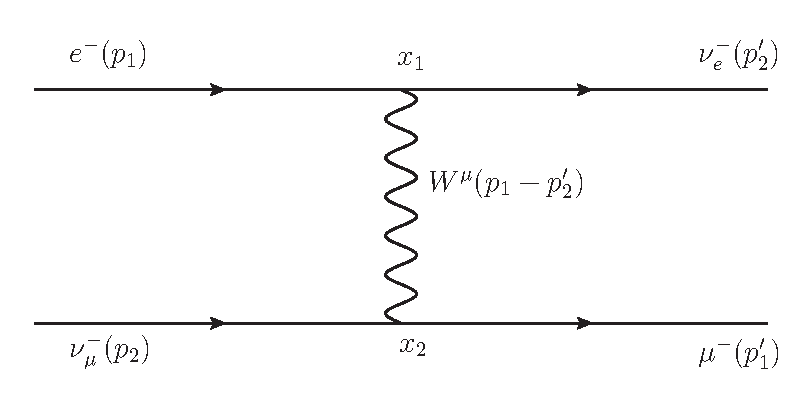
\includegraphics{scatteringw} %noinstiki
  \caption{scattering with four fermions} %noinstiki
  \label{fig:sw} %noinstiki
\end{figure} %noinstiki
Therefore we have

\begin{align}
  \mathcal{M}_{fi}=\frac{G_F}{\sqrt{2}}
\bar{u}_{\nu_e}(\mathbf{p}_2')\gamma^\mu(1-\gamma_5)u_e(\mathbf{p_1})
\bar{u}_\mu(\mathbf{p}_1')\gamma_\mu(1-\gamma_5)u_{\nu_\mu}(\mathbf{p_2})
\end{align}
We now must sqaure the scattering amplitude, $\mathcal{M}$, and summing up over final spin states, and averaging over the intial spin states, as we did in Eq.~\eqref{eq:81f}. The result that will be obtained in detail in Chapter~\ref{cha:three-body-decays} for the muon--decay is
\begin{align}
  \label{eq:102f}
  \overline{|\mathcal{M}|^2}=64\,G_F^2\,(p_1\cdot p_2)(p_1'\cdot p_2')
\end{align}

From Eq.~\eqref{eq:74f}
\begin{align}
  \label{eq:103f}
  \frac{d\sigma}{d\Omega}=\frac{1}{64\pi^2s}\left(\frac{s-m_\mu^2}{s-m_e^2}\right)\overline{|\mathcal{M}|^2}
\end{align}

The center of mass (CM) frame is defined by the condition in Eq.~\eqref{eq:55f}:
\begin{align}
  \mathbf{p}_1+\mathbf{p}_2=0
\end{align}
The $\delta$--function in Eq.~\eqref{eq:101f}
\begin{align}
  \delta^{(4)}(p_1+p_2-p_1'-p_2')=\delta^{(3)}(\mathbf{p}_1+\mathbf{p}_2-\mathbf{p}_1'-\mathbf{p}_2')
\delta(E_1+E_2-E_1'-E_2')
\end{align}

implies
\begin{align}
  \label{eq:157f}
  \mathbf{p}_1+\mathbf{p}_2-\mathbf{p}_1'-\mathbf{p}_2'=0 \overset{\text{CM}}{\Rightarrow}
  \begin{cases}
    \mathbf{p}_1=-\mathbf{p}_2\\
    \mathbf{p}_1'=-\mathbf{p}_2'\\
  \end{cases}
\end{align}
Moreover
\begin{align}
  \sqrt{s}=E_1+E_2
\end{align}
In the CM frame
\begin{align}
\label{eq:104f}
s=&\left(E_1+E_2\right)^2\nonumber\\
=&\left(\sqrt{\mathbf{p}_1^2+m_1^2}+\sqrt{\mathbf{p}_2^2+m_2^2}\right)^2\nonumber\\
=&\left(\sqrt{\mathbf{p}_1^2+m_e^2}+\sqrt{\mathbf{p}_1^2+m_{\nu_e}^2}\right)^2
\end{align}
Therefore
\begin{align}
  \label{eq:105f}
  E_2=|\mathbf{p}_1|
\end{align}
We already have the expression for $|\mathbf{p}_1|$ as given in eq.~\eqref{eq:71f}. In this case $m_2=0$, and $m_1=m_e$, so that
\begin{align}
  \label{eq:158f}
  |\mathbf{p}_1|=\frac{s-m_e^2}{2\sqrt{s}}
\end{align}

From \eqref{eq:105f}
\begin{align}
  \sqrt{s}=&E_1+E_2\nonumber\\
  =&E_1+|\mathbf{p}_1|
\end{align}
\begin{align}
  \label{eq:106f}
  E_1=&\sqrt{s}-|\mathbf{p}_1|\nonumber\\
  =&\sqrt{s}+\frac{-s+m_e^2}{2\sqrt{s}}\nonumber\\
  =&\frac{2s-s+m_e^2}{2\sqrt{s}}\nonumber\\
  =&\frac{s+m_e^2}{2\sqrt{s}}
\end{align}
Then, by using Eqs.~\eqref{eq:157f}, \eqref{eq:105f} and \eqref{eq:158f}, and~\eqref{eq:106f},  we have
\begin{align}
  p_1\cdot p_2=&E_1E_2-\mathbf{p}_1\cdot\mathbf{p}_2\nonumber\\
  =&E_1|\mathbf{p}_1|+\mathbf{p}_1^2\nonumber\\
=&\frac{(s-m_e^2)(s+m_e^2)}{4s}+\frac{(s-m_e^2)^2}{4s}\nonumber\\
=&\frac{(s-m_e^2)}{4s}(s+m_e^2+s-m_e^2)\nonumber\\
=&\frac{1}{2}(s-m_e^2) 
\end{align}
As $p_2^2={p_2'}^2=0$, we have from $\delta$--function
\begin{align}
  (p_1+p_2)^2=&(p_1'+p_2')^2\nonumber\\
  (p_1+p_2)^2=&(p_1'+p_2')^2\nonumber\\
  p_1^2+2p_1\cdot p_2+p_2^2=&{p_1'}^2+2p_1'\cdot p_2'+{p_2'}^2\nonumber\\
  p_1^2+2p_1\cdot p_2=&{p_1'}^2+2p_1'\cdot p_2'\nonumber\\
  m_e^2+2p_1\cdot p_2=&m_\mu^2+2p_1'\cdot p_2'
\end{align}
\begin{align}
  p_1'\cdot p_2'=p_1\cdot p_2-\frac{1}{2}(m_\mu^2-m_e^2)
\end{align}
\begin{align}
  p_1'\cdot p_2'=\frac{1}{2}(s-m_\mu^2) 
\end{align}
Replacing back in Eq.~\eqref{eq:102f} and then in Eq.~\eqref{eq:103f} we have
\begin{align}
  \frac{d\sigma}{d\Omega}=\frac{1}{64\pi^2s}\left(\frac{s-m_\mu^2}{s-m_e^2}\right)
64G_F^2\frac{1}{2}(s-m_e^2)\frac{1}{2}(s-m_\mu^2)
\end{align} 
\begin{align}
    \frac{d\sigma}{d\Omega}=\frac{G_F^2}{4\pi^2}\frac{(s-m_\mu^2)^2}{s}
\end{align}
\begin{align}
\sigma  =\frac{G_F^2}{\pi}\frac{(s-m_\mu^2)^2}{s}
\end{align}
Note that $\sigma\propto s$.
%\left(\right)
%\left[\right]


%%% Local Variables: 
%%% mode: latex
%%% TeX-master: "beyond"
%%% End: